\documentclass[11pt,a4paper]{article}
\usepackage[utf8]{inputenc}
\usepackage[T1]{fontenc}
\usepackage{amsmath}
\usepackage{bigstrut}
\usepackage{amsfonts}
\usepackage[dvipsnames,table,xcdraw]{xcolor}
\usepackage{amssymb}
\usepackage{caption}
\usepackage{hyperref}
\usepackage{titlesec}
\usepackage{siunitx}
\usepackage{booktabs}
\usepackage{array}
\newcolumntype{C}[1]{>{\centering\arraybackslash}m{#1}}
\usepackage{multirow}
\usepackage{subcaption}
\usepackage{hhline}
\usepackage{wrapfig}
\usepackage{lscape}
\usepackage{rotating}
\usepackage[spanish]{babel}
\usepackage[section]{placeins}
\usepackage{tablefootnote}
\usepackage{graphicx}
\usepackage{epstopdf}
\usepackage[font=scriptsize,labelfont=bf]{caption}
\usepackage{anysize}
\marginsize{3cm}{3cm}{2.5cm}{2.5cm}
\providecommand{\abs}[1]{\lvert#1\rvert}
\providecommand{\norm}[1]{\lVert#1\rVert}
\renewcommand{\thesubsection}{\thesection.\alph{subsection}}
\author{Emanuel Alfredo Cortez Médici}
\title{Trabajo Práctico 1}
\DeclareGraphicsExtensions{.jpg,.png}
\usepackage{float}
\usepackage{fancyhdr}
\hypersetup{
    colorlinks,
    linkcolor={red!50!black},
    citecolor={blue!50!black},
    urlcolor={blue!80!black}
}

\urlstyle{same}
\pagestyle{fancy}
\fancyhf{}
%\lhead[\leftmark]{\leftmark}
\rhead[\thepage]{\thepage}

\usepackage{pifont}

\usepackage{soul}
\setstcolor{red}
\setulcolor{red}
\usepackage[tablename=Tabla]{caption}



\begin{document}
	\begin{titlepage}
	\centering
	
	
\includegraphics[width=0.1\textwidth]{fotos_ema/unsl.png} 
	
	{\scshape\LARGE Universidad Nacional de San Luis\par}
	{\scshape Facultad de Ciencias Físico Matemáticas y Naturales.\par}
	{\scshape Ingeniería Electrónica con O.S.D.\par}
	\vspace{1.5cm}
	{\scshape\Large  \par}
	\vspace{1.5cm}
	{\huge\bfseries  Proyecto de diseño y cálculo de una sección de red de telecomunicaciones apta para brindar servicios triple play. \par}

	\vspace{2cm}
	Alumnos\par
	{\Large\itshape Delle Donne Julián \par 
	Toranzo Deivi \par 
	Cortez Médici Emanuel\par}
	\vfill
	Profesores Responsables\par
	Ing. Alfredo ~\textsc{Debattista}\\
	Ing. Sergio ~\textsc{Hernandez} \\
	Ing. Marwan ~\textsc{Geraiges}
	
	\vfill

% Bottom of the page
	{\large \today\par}
\end{titlepage}

\newpage

\tableofcontents

\clearpage
\part{Introducción}

El presente proyecto pretende analizar y diseñar una red de telecomunicaciones capaz de brindar un servicio de triple play en la localidad de  Leandro N. Alem, presente en el noreste de la provincia de San Luis, Argentina. El proveedor se encuentra en la localidad de Quines de la provincia de San Luis.

Se denomina Triple Play al paquete conjunto de servicios de conexión telefónica, televisiva y a Internet. El servicio Triple Play es un término de marketing que utilizan los operadores de telecomunicaciones para ofertar, a través de una única conexión de banda ancha, tres servicios como son acceso a Internet de banda ancha, televisión y teléfono fijo.

Para poder brindar el servicio, teniendo en cuenta la distancia entre las dos localidades, se necesita implementar dos redes: una red de transporte, que unirá ambas localidades, y una red de acceso, que se encargará de distribuir el servicio dentro de la localidad de Leandro N. Alem.

En el análisis se evaluarán aspectos técnicos, socioeconómicos y geográficos, considerando:

\begin{itemize}
    \item topografía y climatología de la zona
    \item situación socioeconómica de la zona
    \item actividad productiva principal y distribución etaria
    \item servicios existentes y competidores
    \item instalación y mantenimiento de los equipos
    \item penetración del servicio y costos de instalación
\end{itemize}

Una vez realizado el estudio se podrá determinar la mejor solución en cuanto al trayecto del enlace, distribución del servicio, flujo de datos, equipamiento necesario, infraestructura e inversión a realizar para poder por último determinar la rentabilidad del proyecto.

\clearpage
\part{Análisis demográfico y socioeconómico}

\section{Departamento de Ayacucho}
Tiene 9.681 km$^2$ y limita al este con los departamentos de Junín y San Martín, al sur con los de Coronel Pringles y Belgrano, al oeste con las provincias de Mendoza y San Juan, y al norte con las de San Juan, La Rioja y Córdoba, lo que lo convierte en el único departamento de la Argentina que limita con cuatro provincias.

\section{Localidad de Leandro N. Alem.}

Leandro N. Alem es una localidad del departamento Ayacucho, en el norte de la provincia de San Luis, Argentina, situada a 110 kilómetros de la ciudad capital de San Luis.


\section{Análisis demográfico}
Según el censo del Instituto Nacional de Estadísticas y Censos (I.N.D.E.C.) del año 2010, el departamento de Ayacucho presenta una población total de 19.613 habitantes. De este departamento se desea analizar particularmente la localidad de Leandro N. Alem, ya que en esta se pretende brindar el servicio. De dicho censo, se obtuvo que la localidad de Leandro N. Alem contaba en el año 2.010 con 379 habitantes, lo que representa un incremento del 30$\%$ frente a los 291 habitantes censados con el censo anterior.

Debido a que se necesita un análisis actual de la situación poblacional de la localidad, se presentará en cada tabla una estimación al actual año 2.021. Para ello, se utilizará una proyección poblacional estimada del departamento de Ayacucho, realizada por la Dirección Provincial de Estadísticas y Censos de la provincia de San Luis. En la misma, se indica que la población total para julio de 2.021 será de 22.266 habitantes. Para estimar la población presente en julio del año 2.021 en la localidad de Leandro N. Além se tuvo en consideración el porcentaje de personas que representaba dicha localidad respecto del departamento de Ayacucho teniendo en cuenta el censo del año 2.010.

Para entonces, Leandro N. Alem representaba el 1,93$\%$ de la población total del departamento Ayacucho. 
Esta conclusión se obtiene de la ecuación \ref{eq:porc_alem}.

\begin{equation}
    \frac{\text{Población de Leandro N. Alem en el año 2.001}}{\text{Población del departamento Ayacucho en el año 2.001}}*100\%=\frac{379}{19613}*100\%=1.93\%
    \label{eq:porc_alem}
\end{equation}

Contrastando con lo que sucedía en el año 2001, se observa que la población de Leandro N. Alem en aquel año representaba el 1,72\% del departamento de Ayacucho,
por lo tanto se puede estimar la población actual utilizando el porcentaje calculado del año 2010, ya que no se percibe una variación importante entre décadas. 
Teniendo en cuenta que la población correspondiente al año 2.021 para el departamento de Ayacucho es de 22.266 personas y suponiendo que se mantuvo constante el porcentaje de la población que reside en Leandro N. Alem, la cantidad de personas estimada para el año 2.021 es de 430 personas. 
Gracias a declaraciones de la intendencia, se pudieron corroborar estas suposiciones. 
Estos resultados se presentan en la tabla \ref{tab:habitantes_futur_alem}.

\begin{table}[htbp]
 \resizebox{\textwidth}{!}{%
  \centering
  
    \begin{tabular}{|c|p{0.25\linewidth}|p{0.25\linewidth}|p{0.25\linewidth}|}
    \hline
    Lugar & Cantidad de habitantes para el año 2.001 & Cantidad de habitantes para el año 2.001 & Cantidad de habitantes para el año 2.021 \\
    \hline
    Ayacucho & 16906 & 19613 & 22266 \\
    \hline
    Leandro N. Alem & 291  & 379  & 430 \\
    \hline
    \end{tabular}}%
    \caption{cantidad de habitantes en el año 2.010 y previstos para julio del 2.021 en la localidad de Leandro N. Alem.}
  \label{tab:habitantes_futur_alem}%
\end{table}%


Gracias a los datos aportados por el censo del I.N.D.E.C. y la estimación de la Dirección Provincial de Estadísticas y Censos de la Provincia de San Luis, se pueden analizar la cantidad de hogares con necesidades básicas insatisfechas en ambas localidades y la cantidad de personas por hogar.

Por otro lado, el I.N.D.E.C. brinda además información sobre la cantidad de usuarios que poseen computadoras, teléfonos fijos y teléfonos celulares. 
Dicha información se presenta en la Tabla 5.
Esta información es de particular interés, ya que es necesaria para determinar los posibles usuarios del servicio que se desea brindar.
Se presenta juntamente, una cantidad actual supuesta.
Para ello, se utilizaron los datos brindados por el I.N.D.E.C., los cuales mostraban que al cuarto trimestre del año 2019, el 79,9$\%$ de la población argentina tenía acceso a internet.
Además, entre el cuarto trimestre de 2019 y el cuarto trimestre de 2020, se produjo un crecimiento interanual en la utilización de internet del 1,1$\%$.
Por lo tanto, esto resulta en que el 80,78$\%$ de la población utiliza actualmente internet.
Debido a que se necesitan de estos dispositivos para acceder a internet, es que se puede suponer que la cantidad de los mismos aumentó en la misma proporción.

Los datos recabados y previstos son mostrados en la tabla \ref{tab:prediccion_alem}.


\begin{table}[htbp]
  \centering
    \begin{tabular}{|p{0.45\linewidth}|c|c|}
    \hline
    Localidad & \multicolumn{2}{|c|}{Leandro N. Alem} \\
    \hline
    Año  & 2010 & Previsión 2021 \\
    \hline
    Población & 379  & 430 \\
    \hline
    Población con necesidades básicas insatisfechas & 12   & 14 \\
    \hline
    Cantidad de personas por hogar & 3    & 3 \\
    \hline
    Cantidad de personas que poseen computadoras, teléfonos fijos o teléfonos celulares & 132  & 347 \\
    \hline
    \end{tabular}%
    \caption{análisis demográfico en la localidad de Leandro N. Alem.}
  \label{tab:prediccion_alem}%
\end{table}%


Una vez definidos los distintos habitantes y hogares que pueden satisfacer sus necesidades básicas, es necesario agrupar aquellos que poseen características en común para así poder determinar los tipos de servicios que se pueden brindar.

Una característica importante para determinar el modelo de consumo, es la edad.
Dependiendo de la edad, existirán o no requerimientos mayores en el servicio de internet y/o televisión.
Por dicho motivo se analizarán 3 grupos etarios, personas entre 25 y 35 años, personas entre 35 y 60 años y personas mayores de 60 años. 
Esta elección en la división se realizó teniendo en cuenta características en común en dichas franjas etarias, siendo todas personas que generalmente están en edad de trabajar o de recibir un sueldo, si es que los mismos son jubilados.

Para la edad entre 25 y 35 años, se encontró que en el 2.001 existían en Leandro N. Alem 20 personas en dicho rango etario, representando el 6,9$\%$ del total. 
Para el año 2.010, esta cantidad aumentó a 48 personas, representando el 12,7$\%$ del total.
Debido a la gran variabilidad en la composición etaria que suelen presentar los pueblos, es que a pesar del aumento abrupto en la proporción a lo largo del periodo 2.001-2.010, es que se decide utilizar el porcentaje obtenido con el censo del año 2.010 y trasladarlo al año 2.021 sin aumentarlo.
Realizando esto, se estima que existen 55 personas entre 25 y 35 años.

Para la edad entre 35 y 60 años, se encontró que en el 2.001 existían 88 personas en dicho rango etario, los cuales conformaban el 30,2\% de la población total. En el año 2.010, existían 105 personas, conformando el 27,7\% del total.
Debido a que la variación no fue significativa en el periodo entre décadas, se utiliza el mismo porcentaje que el obtenido para el año 2.010. 
Con dicha consideración, se estima que en la actualidad existen 119 personas pertenecientes a dicho rango etario.

Finalmente, para el grupo etario de mayores de 60 años, se obtuvo que en el año 2.001 existían 70 habitantes, representando el 24$\%$ del total poblacional, mientras que en el año 2.010 existían 79 personas, representando el 20,8$\%$. A pesar de la reducción en este grupo, se prefiere continuar con este porcentaje para la estimación del año 2.021.
Con el porcentaje mencionado, se obtuvo que existen en Leandro N. Alem 89 habitantes mayores a 60 años.
Los datos previamente calculados se muestran en la tabla \ref{tab:etario_alem}.

Con dichos datos, se podrán determinar distintos grupos a los cuales brindar un servicio adecuado a sus necesidades e intereses.



\begin{table}[htbp]
  \centering
    \begin{tabular}{|p{0.3\linewidth}|c|c|}
    \hline
    Localidad & \multicolumn{2}{|c|}{Leandro N. Alem} \\
    \hline
    Año  & 2010 & Previsión 2021 \\
    \hline
    Personas entre 25 y 35 años & 20   & 48 \\
    \hline
    Personas entre 35 y 60 años & 88   & 105 \\
    \hline
    Personas mayores a 60 años & 70   & 79 \\
    \hline
    \end{tabular}%
  \caption{análisis de los distintos grupos etarios en la localidad de Leandro N. Alem.}
  \label{tab:etario_alem}%
\end{table}%

\section{Análisis económico}

Observando la Fig. \ref{fig:agropecuaria} y la Fig. \ref{fig:industria}, se puede concluir que la principal actividad privada que se desarrolla en el departamento Ayacucho es la actividad agropecuaria.

\begin{figure}[ht!]
  \centering
  \subcaptionbox{actividad agropecuaria por departamento.\label{fig:agropecuaria}}%
  [.45\linewidth]{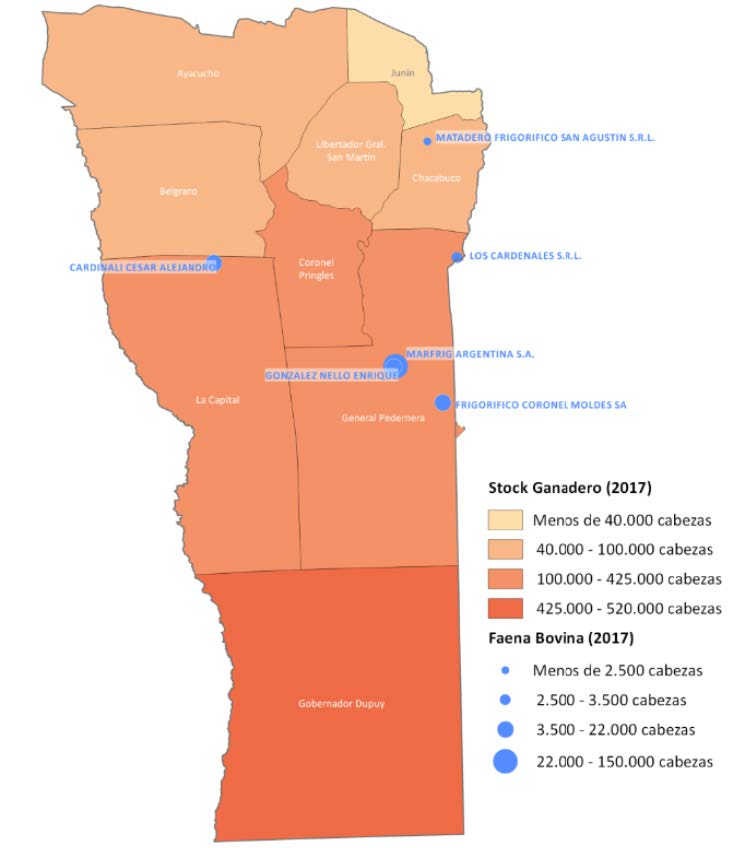
\includegraphics[height=15\baselineskip]{fotos_ema/agropecuaria}}
\subcaptionbox{actividad industrial por departamento.\label{fig:industria}}
  [.45\linewidth]{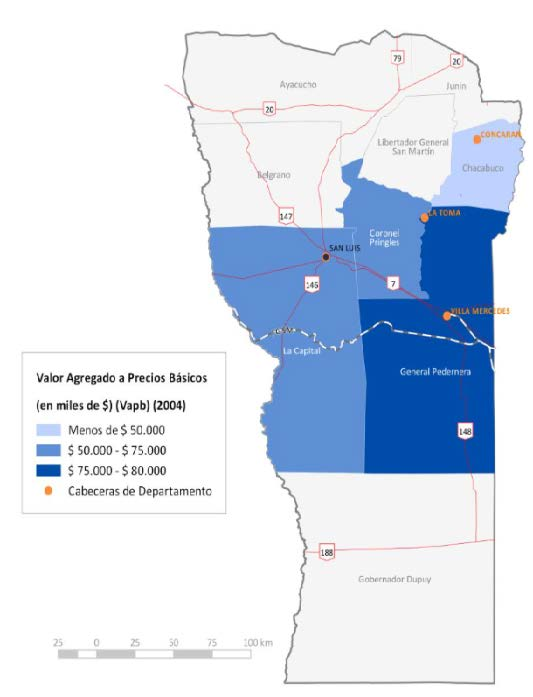
\includegraphics[height=15\baselineskip]{fotos_ema/industria}}
  \caption{actividades económicas de la provincia de San Luis por departamento.}
  \label{fig:econo_deptos}
\end{figure}

Por lo tanto, si se tienen en cuenta los datos aportados por la tabla \ref{tab:salarios_alem}, para el año 2.017 se tiene un sueldo de \$17.691. 
Tomando en cuenta que la inflación acumulada en los años 2.017, 2.018, 2.019 y 2.020 es del 162,3\%, se puede determinar que el valor actual ajustado por inflación corresponde a \$46.403 pesos argentinos para el sector privado.

Por otro lado, el sector público, el cual representa el 16\% de la población total, y el 35,5\% de la población laboralmente activa, poseía al año 2017 un sueldo promedio de \$24.172. 
Teniendo en cuenta la inflación acumulada mencionada anteriormente, se puede determinar que el valor actual ajustado por inflación corresponde a \$63.403 pesos argentinos para el sector público.

Finalmente, se puede determinar que el sueldo promedio general que se considerará será de \$52.470. Esto se obtuvo de la ecuación \ref{eq:sueldo_promedio_alem}.


\begin{equation}
    \$63403*35.5\% + \$46403*64.5=\%52.470
    \label{eq:sueldo_promedio_alem}
\end{equation}


Tomando en cuenta la cantidad de personas por hogar, mostradas en la Tabla 4, se puede determinar un grupo familiar formado por 1 matrimonio y 1 hijo, el cual puede presentar como ingreso un sueldo general, previamente desarrollado.
La ventaja de considerar este tipo de grupo con una sola fuente de ingreso es que puede nuclear también una familia monoparental.
Debido a que este grupo incluye un ingreso el cual puede ser proveniente tanto del sector público o privado, se puede suponer que este representa el 50\% de la población laboralmente activa, es decir la población entre 25 y 60 años.
Considerando esto, este grupo representa el 33,1\% de la población que recibe un ingreso.
Otro grupo a considerar es un matrimonio de jubilados, suponiendo que ambos cobran la jubilación mínima, esto da un ingreso total de \$41.142. 
Del análisis anterior se puede suponer que este grupo representa el 20,7\% de la población total, y el 33,8\% de la población que percibe un ingreso, analizada previamente. 
Un tercer grupo familiar a tener en cuenta es el conformado por 2 fuentes de ingreso, suponiendo que una proviene de trabajar en el sector privado y otra de trabajar en el sector público. 
Esto da un ingreso total de \$109.806.
Debido a lo analizado previamente, la proporción de este grupo se puede estimar teniendo en cuenta el porcentaje restante de la población que percibe un ingreso, dando cómo resultado una proporción del 33,1\%. Estos datos se presentan en la tabla \ref{tab:grupos_sueldos_alem}.


\begin{table}[htbp]
  \resizebox{\textwidth}{!}{%
  \centering
    \begin{tabular}{|p{0.25\linewidth}|p{0.25\linewidth}|p{0.25\linewidth}|p{0.25\linewidth}|}
    \hline
    Sector & Rama de actividad & Salario en pesos promedio en el año 2.017 & Salario en pesos previsto para el año 2021 \\
    \hline
    Privado & Agricultura, ganadería y pesca & \$17.691 & \$46.403 \\
    \hline
    Público & Servicios & \$24.172 & \$63.403 \\
    \hline
    \end{tabular}}%
      \caption{salario en pesos promedio en 2.017 y previsto para 2.021.}
  \label{tab:salarios_alem}%
\end{table}%




\begin{table}[htbp]
  \resizebox{\textwidth}{!}{%
  \centering
    \begin{tabular}{|p{0.3\linewidth}|p{0.3\linewidth}|p{0.3\linewidth}|}
    \hline
    Grupos & Sueldo considerado & Porcentaje aproximado de la población que percibe un ingreso \\
    \hline
    Grupo familiar con una sola fuente de ingreso & \$ 52.470 & 33,10\% \\
    \hline
    Jubilados & \$ 41.142 & 33,80\% \\
    \hline
    Grupo familiar con dos fuentes de ingreso & \$ 109.806 & 33,10\% \\
    \hline
    \end{tabular}}%
  \caption{resumen de los distintos grupos económicos.}
  \label{tab:grupos_sueldos_alem}%
\end{table}%


Un indicador fundamental para determinar el porcentaje de la población que podrá acceder a nuestros servicios fue el de Necesidades Básicas Insatisfechas (N.B.I.). 
El mismo permite identificar características críticas en la población y delimitar grupos de pobreza que no tienen los ingresos suficientes para pagar nuestro servicio. 
Según las estadísticas mostradas en la Tabla 3 , se registraron 12 personas con NBI en la localidad de Leandro N. Alem en el año 2.010, representando el 3,16\% de la población total.

Haciendo uso de la proyección poblacional estimadas anteriormente al año 2.021 y teniendo en cuenta que las siguientes consideraciones quedan excluidas del razonamiento:

\begin{itemize}
    \item La pandemia causada por el COVID 19
    \item La tasa inflacionaria del país
    \item Las diversas crisis económicas que atravesó el país
    \item Corrida cambiaria y desestímulo a la inversión privada
\end{itemize}

Se puede realizar entonces una estimación del índice de NBI que presenta la localidad en la actualidad, considerando que este se mantiene constante a lo largo de la década. 
Esto da como resultado un total de 14 personas con NBI. 
Si bien esta no es la mejor aproximación, se optó por utilizarla de referencia dado que no se pudo encontrar información actualizada sobre este índice.

En la tabla 4 se puede observar la cantidad promedio de personas por hogar que había en el año 2.010, siendo esta de 3 personas. 
Si consideramos que en la actualidad el promedio de personas por hogar sigue siendo el mismo, y teniendo en cuenta que la población total estimada para el año 2.021 fue de 430 habitantes, se puede calcular la cantidad de hogares a partir de la ecuación \ref{eq:hogares_alem}, dando como resultado 144 hogares.

\begin{equation}
    \frac{\text{Población de Leandro N. Alem en el año 2.021}}{\text{Cantidad de personas por hogar}}=\frac{430}{3}=144
    \label{eq:hogares_alem}
\end{equation}


Siguiendo el mismo razonamiento descrito anteriormente se puede calcular la cantidad de hogares con NBI en la localidad de Leandro N. Além, dando como resultado un total de 5 hogares con NBI. Debido a que no pueden cubrir sus necesidades básicas, lamentablemente no se podrán considerar en la prestación del servicio. 
Esto deja disponible la cantidad de 139 hogares para brindar el servicio.

\section{Análisis competitivo}

Debido a que la provincia de San Luis cuenta con antenas Wi-Fi públicas, es menester analizar si estás proveen de buen internet a la zona o si el servicio está saturado. 
Sin embargo, haciendo uso del sitio web nperf.com, se puede corroborar que en esta localidad no se encuentran antenas de ningún proveedor de telefonía móvil (Claro, Personal o Movistar) lo que favorece a la hora de buscar posibles consumidores. 
Por otro lado, cabe destacar la inexistencia de proveedores de televisión por cable. 
El servicio de TV llega solamente a través de la empresa DirecTV. 
Por lo tanto, se procederá a realizar un relevamiento tanto del servicio de internet brindado por el estado, así como los posibles precios que maneja DirecTV.


\subsection{Wi-Fi público}

En la localidad de Leandro N. Alem, se encuentran presentes 4 antenas Wi-Fi, tal como se observa en la Fig. 3.
De estas 4 antenas, 3 trabajan con una frecuencia de 2,4 GHz, mientras que sólo una trabaja con 5 GHz.
Analizando el uso de las antenas en horarios picos, se obtuvo un promedio de 34 usuarios por antena.
Considerando el tipo de antena predominante y la cantidad de usuarios por antena, se puede concluir que, efectivamente, el servicio de internet público se encuentra saturado, prestando la oportunidad de brindar una alternativa de pago que ofrezca un mejor comportamiento.

\subsection{DirecTV}

Debido a la falta de televisión por cable, la televisión satelital es la única opción con la que disponen los habitantes de Leandro N. Alem, siendo la opción de pago más extendida en Argentina DirecTV. 
Observando los precios en la página oficial de DirecTV, se tiene que el servicio básico tiene un precio de \$2.098, con 145 canales HD, mientras que el mejor servicio posee un precio de \$3.393, con 255 canales HD 4K.
Es por ello, que al analizar los precios que se desearán manejar, se deberá respetar este margen de precios.
No obstante, a pesar de la gran oferta brindada por este servicio, un talón de Aquiles presente es la inestabilidad del servicio ante las inclemencias del tiempo, tales como vientos, muy presentes en la zona, o lluvias.
Esto deja margen a que, si se puede brindar un servicio que sea estable, incluso con una oferta menor, se pueda competir fácilmente con el prestador dominante.

\subsection{Características del servicio que se desea brindar}

Mediante el análisis demográfico, se deduce que la mayor parte de Leandro N. Alem es zona rural.
Por lo tanto, se deben tener en cuenta las posibles necesidades de una persona de campo, como por ejemplo: el diario/ agencia de noticias, el canal del clima, canal “La rural”, etc. 
El servicio de Wi-Fi público en hora pico hace imposible el uso de estos sitios web, por lo tanto se debe proveer un servicio con ancho de banda capaz de satisfacer estas necesidades. 
Lo mismo ocurre con el servicio de televisión de Directv en los días de lluvia o vientos fuertes.
Además de poseer un catálogo de canales innecesariamente grande para este tipo de consumidores por lo que se dispondrá tener una cantidad reducida de canales (que contengan los canales anteriormente nombrados).
Luego de los distintos análisis realizados, se procederá a determinar las características del servicio que se pretende brindar en la zona.

\subsection{Televisión}

Se ofrecerán 2 servicios, uno básico con 50 canales SDTV y otro premium con 56 canales, 6 de los cuales serán HDTV y 50 SDTV. 
Se toman 6 canales HD, para cubrir la necesidad de ver canales de deportes y películas en una mejor resolución.

\subsection{Internet}

Junto con el servicio básico, se ofrecerán 6 mbps, mientras que el servicio premium contará con una velocidad de 15 mbps.

\subsection{Precio, contenido y alcance del servicio}

Con el desarrollo del análisis económico, se llega a que el salario promedio de un habitante de Leandro N. Alem es de \$52.470.
Para poder abrirse paso entre la competencia, se considera no cobrar más del 8\% del salario promedio, lo que da un límite de \$4.197.
Además, para no abrumar a los posibles clientes con tantas posibilidades, se pone a disposición solo tres opciones. 
Por lo tanto, los precios de nuestro servicio y su contenido son los mostrados en la tabla \ref{tab:precios}. 
El pack básico que cuenta con un servicio de 50 canales SDTV está pensado para el grupo etario de mayores a 60 años, que según el estudio realizado anteriormente, está conformado por alrededor de 89 personas. 
El pack intermedio tiene como objetivo a familias con uno o dos salarios básicos que quieran acceder a un servicio de internet decente contando además con el servicio de 50 SDTV. 
Por último, el pack premium está destinado a personas con un salario mayor al promedio y quieren adquirir un servicio de internet y televisión de buena calidad.
Al ser este un sector más reducido se estima que será el pack que menos se contrate.


\begin{table}[htbp]
  \centering
    \begin{tabular}{|c|c|c|}
    \hline
    Tipo de pack & Contenido & Precio en pesos \\
    \hline
    Básico & 50 SDTV & \$1500 \\
    \hline
    Intermedio & 50 SDTV+6 mbps &  \$2800 \\
    \hline
    Premium & 50 SDTV+6 HDTV+15 mbps & \$4000 \\
    \hline
    \end{tabular}%
  \caption{precios del servicio}
  \label{tab:precios}%
\end{table}%



Considerando que los hogares con N.B.I harán uso del Wi-fi público y que no todos los habitantes van a querer adquirir alguno de los packs propuestos ya que un porcentaje de la población optará por continuar usando la red pública y aprovechar la migración de usuarios a este nuevo servicio, esto ocasionará un alivio en la red, convirtiéndola en una red utilizable si solo se conecta un 40\% (alrededor de 41 personas por antena) de la población tenida en cuenta para los análisis previos.
Por otro lado, el porcentaje de la población que es cliente de DirecTV optará por adquirir este nuevo servicio al tener un precio menor y mayor fiabilidad frente a los cambios climáticos.
Por lo tanto, el porcentaje de población que adquirirá este servicio es del 60\%, dando un total de 83 hogares.



\section{Modelo de consumo}

Del estudio socioeconómico realizado se obtuvo como conclusión que 83 hogares del total de la población de la localidad de Leandro N. Alem serían potenciales clientes. 
En base a este resultado se procede a calcular el ancho de banda total de cada servicio proporcionado y en consecuencia el ancho de banda total que deberá soportar la red troncal.

\subsection{TV}

En la tabla \ref{tab:tv_maxima} se observa la máxima cantidad simultánea para cada tipo de servicio que se ofrece y su correspondiente ancho de banda. Multiplicando la mayor cantidad de canales de cada tipo (SDTV y HDTV) por su correspondiente ancho de banda se obtiene la tasa de bit necesaria para la transmisión del servicio de TV.
Esto se muestra en la ecuación \ref{eq:tasa_bits_tv}.

\begin{equation}
    \text{Tasa de bits: } 50*1.5*10^6+6*6*10^6=111 \text{ Mbps}
    \label{eq:tasa_bits_tv}
\end{equation}

No se considera necesaria la utilización de buffer ya que se transmitirán solo 56 canales.

\begin{table}[htbp]
  \centering
    \begin{tabular}{|c|c|c|}
        \hline 
        \textbf{Servicio} & \textbf{Ancho de banda} & \textbf{Cantidad Máx. simultánea} \\ \hline 
        \textbf{Canal SDTV} & 1.5 Mbps & 50 \\ \hline 
        \textbf{Canal HDTV} & 6 Mbps & 6 \\ \hline 
        \textbf{VoIP} & 30 kbps & 83 \\ \hline 
        \textbf{Internet} & 6/15 Mbps & 44/14 \\ \hline 
    \end{tabular}
  \caption{Cantidad máxima simultánea vs. ancho de banda}
  \label{tab:tv_maxima}%
\end{table}%


\subsection{VoIP}

La mayor cantidad de clientes que pueden estar usando nuestro servicio es igual a la cantidad de hogares, multiplicando por el ancho de banda que muestra la tabla \ref{tab:tv_maxima} se obtiene un total de 1,92 Mbps. Esto se muestra en la ecuación \ref{eq:tasa_bits_tel}.

\begin{equation}
    \text{Tasa de bits: } 83*30*10^3=1.92 \text{ Mbps}
    \label{eq:tasa_bits_tel}
\end{equation}

Se puede observar que la tasa de bit correspondiente a la transmisión del servicio VoIP es mucho menor al de TV siendo este despreciable a la hora de considerar el ancho de banda total que deberá soportar la red troncal .

\subsection{Internet}
Con los resultados obtenidos previamente se hicieron estimaciones de cuántas personas podrían optar por contratar los pack intermedios y premium que prestan un servicios de 6 y 15 Mbps respectivamente. 
Se consideró realizar un porcentaje de cuántos clientes podrian optar por cada pack en base a su clasificación económica/familiar (familias con uno o dos sueldos y jubilados).
También se consideró la disponibilidad de las antenas de Autopista de la Información que brindan internet en la zona. 
Con este razonamiento en mente se estimaron los resultados de la tabla \ref{tab:porcent_total_packs} donde el 53\% de los 83 posibles clientes optará por el pack intermedio y el 17\% por el pack premium dando como resultado un total de 44 y 14 clientes respectivamente como muestra la tabla \ref{tab:tv_maxima}. 



\begin{table}[htbp]
\resizebox{\textwidth}{!}{%
  \centering
    \begin{tabular}{|c|c|c|c|c|}
    \hline 
    \textbf{Grupo} & \textbf{Pack Básico $[\%]$ } & \textbf{Pack intermedio $[\%]$} & \textbf{Pack premium $[\%]$} & \textbf{Total de grupo $[\%]$} \\ \hline 
    \textbf{Familias con un sueldo} & 4 & 25,1 & 4 & 33.1 \\ \hline 
    \textbf{Familias con dos sueldos} & 2 & 19,1 & 12 & 33.1 \\ \hline 
    \textbf{Jubilados} & 24 & 8,8 & 1 & 33.8 \\ \hline 
    \textbf{Total} & 30 & 53 & 17 & 100 \\ \hline 
    \end{tabular}}
  \caption{porcentaje total de cada grupo que optara por cada uno de los packs.}
  \label{tab:porcent_total_packs}%
\end{table}%


Multiplicando esta cantidad de clientes por el ancho de banda se obtiene la tasa de bit necesaria para el servicio de internet. Esto se muestra en la ecuación \ref{eq:tasa_bits_internet}

\begin{equation}
    \text{Tasa de bits: } 44*6*10^6+14*15*10^6=474 \text{ Mbps}
    \label{eq:tasa_bits_internet}
\end{equation}

 En la tasa de bits correspondiente al utilizado por la red de internet, a diferencia del servicio de TV y VoIP, se considera que no se utiliza el 100\% del ancho de banda. 
 Esto no sucede en la práctica ya que se producen pausas en el tráfico que reducen el uso del ancho de banda. 
 Además, no todos harán uso del servicio de internet al mismo tiempo y en cada caso varía la utilidad que le dan, no siendo lo mismo hacer una videollamada que solo mandar un mensaje de texto o un mail. 
 Teniendo esto en cuenta y además de que Leandro N. Alem es un pueblo pequeño, mayormente agrícola, se considera utilizar un factor de simultaneidad del 30\%.
 Con este factor de simultaneidad se estima poder ofrecer un servicio estable a los usuarios.
 El resultado es una tasa de bits total de 255 Mbps como muestra la ecuación \ref{eq:tasa_de_bits_total}, la cual deberá soportar la red troncal.
 
 \begin{equation}
     \text{Tasa de bits: } 111*10^6+1.92*10^6+142.2*10^6\approx255 \text{ Mbps}
     \label{eq:tasa_de_bits_total}
 \end{equation}


 \clearpage 

 \part{Red troncal}

\section{Red troncal con radioenlace}

\subsection{Determinación de las frecuencias a utilizar para la transimisión}

Al analizar los datos disponibles en el sitio web del ENACOM\footnote{\href{https://www.enacom.gob.ar/bandas-de-uso-compartido-sin-autorizacion_p680}{Bandas de uso compartido sin autorización}}, se optará por usar una banda de uso compartido sin autorización ya que dispone de bandas de frecuencias óptimas para la utilización de una antena de 5GHz. 
Las bandas de uso compartido sin autorización se rigen mediante la Resolución del Ministerio de Modernización N$\mathrm{{}^\circ}$ 581/ 18\footnote{\href{https://www.argentina.gob.ar/normativa/nacional/resolución-581-2018-314174}{Resolución del Ministerio de Modernización N$\mathrm{{}^\circ}$ 581/ 18}}, la cual establece que las bandas de frecuencias radioeléctricas, detalladas a continuación en la tabla \ref{tab:frec_libres}, se declaran de uso compartido en el ámbito del territorio nacional y no requieren de autorización para su uso, debiendo respetarse las condiciones y parámetros técnicos de emisión establecidas por el Ente Nacional de Comunicaciones en la Resolución N$\mathrm{{}^\circ}$ 4653/19\footnote{\href{https://www.enacom.gob.ar/multimedia/normativas/2019/res4653.pdf}{Resolución N$\mathrm{{}^\circ}$ 4653/19}}:

\begin{table}[htbp]
  \centering
\begin{tabular}{|c|} \hline 
Rango de frecuencias: \\ \hline 
915-928 [MHz] \\ \hline 
2400-2483.5 [MHz] \\ \hline 
5150-5250 [MHz] \\ \hline 
5250-5350 [MHz] \\ \hline 
5470-5600 [MHz] \\ \hline 
5650-5725 [MHz] \\ \hline 
5725-5850 [MHz] \\ \hline 
57000-71000 [MHz] \\ \hline
\end{tabular}
\caption{rango de frecuencias de uso compartido.}
\label{tab:frec_libres}
\end{table}%


Esto genera un ahorro importante a la hora de calcular costos al no tener que licitar una banda de frecuencias. Asimismo, los usuarios de las bandas de frecuencias de uso compartido que operen en la modalidad de uso \textbf{Prestador} deberán notificar al Ente Nacional de Comunicaciones las coordenadas geográficas, altura de antena de las estaciones radiobases que instalen, datos de homologación del equipo y bandas de frecuencia de operación. Dicha notificación deberá tramitarse a través de la plataforma "Trámites a Distancia" (TAD) del sistema de Gestión Documental Electrónica\footnote{\href{https://tramitesadistancia.gob.ar/}{Trámites a distancia}}. Otro punto importante para hacer uso de esta banda de frecuencia es la potencia permitida. Al analizar la Resolución RESOL-2018-581-APN-MM\footnote{\href{https://www.enacom.gob.ar/multimedia/normativas/2018/res581MM.pdf}{Resolución RESOL-2018-581-APN-MM}} se corrobora que la potencia a utilizar está en el rango permitido.

Con esto definido y con la utilización del CABFRA\footnote{\href{https://www.enacom.gob.ar/cuadro-de-atribucion-de-bandas-de-frecuencias-de-la-republica-argentina-cabfra-\_p1588}{Cuadro de atribución de bandas de frecuencias de la República Argentina}}, el rango de frecuencia desde 5,725 GHz a 5,825 GHz, cuyas características se encuentran en la tabla \ref{tab:rango_frec}, está dentro de los parámetros requeridos. 


\begin{table}[htbp]
\resizebox{\textwidth}{!}{%
  \centering
    \begin{tabular}{|p{0.25\linewidth}|p{0.25\linewidth}|p{0.25\linewidth}|p{0.25\linewidth}|}
    \hline
    \multicolumn{4}{|c|}{Rango de frecuencia} \bigstrut\\
    \hline
    \multicolumn{4}{|c|}{\textbf{5.725 - 5.825}} \bigstrut\\
    \hline
    \multicolumn{4}{|c|}{Observaciones generales} \bigstrut\\
    \hline
    \multicolumn{4}{|c|}{} \bigstrut\\
    \hline
    SERVICIO (T10) & TIPO DE SERVICIO & CARACTERÍSTICAS & NORMATIVA \bigstrut\\
    \hline
    Servicio de Radiolocalización - SRL & FIJO/MOVIL &      & RR UIT/R2 - Art. 5 \bigstrut\\
    \hline
    Servicio de Aficionados - SAF & FIJO/MOVIL & Banda de 5 cm & 3635ENACOM17 508ENACOM18 4653ENACOM19 \bigstrut\\
    \hline
    Servicio TIC para banda de frecuencia de uso compartido & FIJO/MOVIL & Uso Privado - Prestador (5.725 - -5.850 MHZ) & 581MM18 4653ENACOM19 \bigstrut\\
    \hline
    Sistemas de Baja Potencia - SBP & FIJO/MOVIL & Categoría Secundaria (3,1 - 10,6 GHz) & 5186ENACOM17 507ENACOM18 \bigstrut\\
    \hline
    \end{tabular}}%
    \caption{características para el rango de frecuencia entre 5.725 y 5.825 MHz.}
  \label{tab:rango_frec}%
\end{table}%

Para conseguir la canalización de la banda de frecuencias a utilizar, se debe consultar con la tabla de asignación de canales de la frecuencia de 5GHz\footnote{\href{https://www.ekahau.com/blog/channel-planning-best-practices-for-better-wi-fi/}{Tabla de asignación de canales de la frecuencia de 5GHz}}. 
De esta tabla se obtiene que este rango de frecuencias posee cuatro canales de 20 MHz, dos de 40 MHz y uno de 80 MHz, como se muestra en la Fig. \ref{fig:canales_frec}.

\begin{figure}[htbp]
\centering
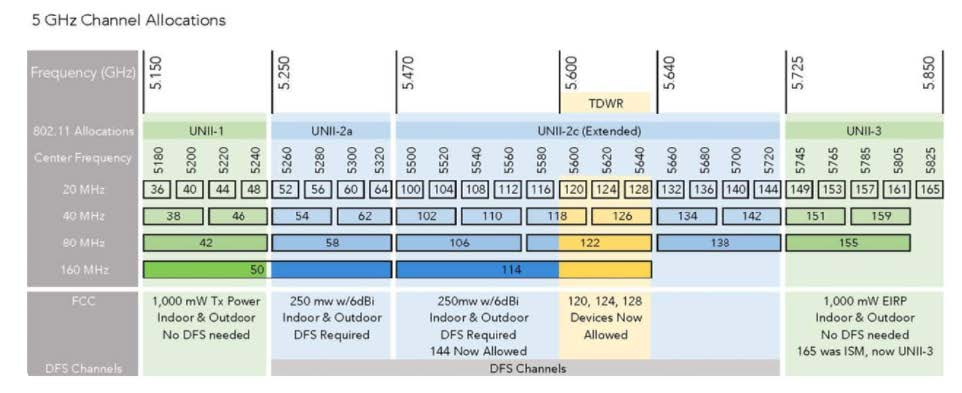
\includegraphics[width=\linewidth]{fotos_ema/canales_frec}
\caption{canales presentes en el rango de frecuencia de 5.725 a 5.825 MHz.}
\label{fig:canales_frec}
\end{figure}

 Al entrar más en detalle en las características de cada canal disponible, se usará el canal 155 que posee las características expuestas en la tabla \ref{tab:carac_155}. 
 Estos datos son sacados del Listado de canales WLAN\footnote{\href{https://en.m.wikipedia.org/wiki/List_of_WLAN_channels}{Listado de canales WLAN}}.

\begin{table}[htbp]
  \resizebox{\textwidth}{!}{%
  \centering
  \begin{tabular}{|c|p{0.25\linewidth}|p{0.25\linewidth}|p{0.25\linewidth}|} 
    \hline 
    Número del canal: & Frecuencia de portadora en MHz: & Rango de frecuencias en MHz: & Ancho de banda del canal en MHz: \\ 
    \hline 
    155 & 5775 & 5735-5815 & 80 \\ 
    \hline 
  \end{tabular}}
\caption{características del canal 155.}
\label{tab:carac_155}
\end{table}

\subsection{Determinación de los equipos para el radioenlace troncal}

Teniendo en cuenta una tasa de transferencia de 255 Mbps, obtenida previamente, y una distancia entre Leandro N. Além y Quines de 35 kilómetros, se consideran los siguientes equipos presentes en la tabla \ref{tab:equipo_tronc_wireless}.
En la misma, se observan las distintas características obtenidas de las hojas de datos de los transmisores y antenas consideradas para conformar la red troncal. 
La opción 1 está formada por el transmisor AirFiber 5X HD y la antena AF-5G34-S45, ambos de la marca Ubiquiti, mientras que la opción 2 está formada por el transmisor B5c de la marca Mimosa y la antena HG5158DP-32D de la marca L-Com.



\begin{table}[htbp]
  
  \centering
  
    \begin{tabular}{|c|c|c|}
\cline{2-3}    \multicolumn{1}{r|}{} & \textbf{Opción 1} & \textbf{Opción 2} \bigstrut\\
    \hline
    \textbf{Transmisor} & AirFiber 5X HD\tablefootnote{\href{https://dl.ubnt.com/datasheets/airfiber/airFiber_5XHD_DS.pdf}{Datasheet AirFiber 5X HD}} & Mimosa B5c \tablefootnote{\href{https://mimosa.co/uploads/datasheets/Mimosa-by-Airspan-B5c-Datasheet_DS-0008-09.pdf}{Datasheet Mimosa B5c}}\bigstrut\\
    \hline
    \textbf{Tasa de transferencia} & 272,64 Mbps & 260 Mbps \bigstrut\\
    \hline
    \textbf{Ancho del Canal} & 80 MHz & 2x80 MHz \bigstrut\\
    \hline
    \textbf{Modulación} & 64 QAM MIMO & 64 QAM MIMO\bigstrut\\
    \hline
    \textbf{Potencia de salida} & 24 dBm & 24 dBm \bigstrut\\
    \hline
    \textbf{Sensibilidad del receptor} & -65 dBm  & -65 dBm \bigstrut\\
    \hline
    \textbf{Frecuencia de operación} & 5735-5815 MHz & 5735-5815 MHz \bigstrut\\
    \hline
    \textbf{Tipo de duplexación} & TDD & FDD \bigstrut\\
    \hline
    \textbf{Distancia alcance máximo} & Hasta 100 km & - \bigstrut\\
    \hline
    \textbf{Antena compatible} & AF-5G34-S45 \tablefootnote{\href{https://dl.ubnt.com/datasheets/airfiber/airFiber_Antennas_DS.pdf}{Datasheet AF-5G34-S45}}& HG5158DP-32D \tablefootnote{\href{https://www.l-com.com/Images/Downloadables/Datasheets/ds_HG5158DP-32D.pdf}{Datasheet HG5158DP-32D}}\bigstrut\\
    \hline
    \textbf{Ganancia de la antena} & 34 dBi & 32 dBi \bigstrut\\
    \hline
    \end{tabular}%
  \caption{características de los equipos a utilizar}
  \label{tab:equipo_tronc_wireless}%
\end{table}%

La tasa de transferencia se elije de tal manera que se puedan tener más de 255 Mbps de transferencia en downstream, que fue la tasa de transferencia que se calculó en la ecuación \ref{eq:tasa_de_bits_total}. 
El ancho del canal se elije teniendo en cuenta el valor que permita la tasa de transferencia deseada, sin aumentar exageradamente la modulación. 
Es por ello que en ambos casos se trabaja con el canal de 80 Mhz.  

Comparando ambos transmisores, se tiene que la opción 1 posee mejores prestaciones, ya que permite usar un ancho de canal hasta 100 MHz, mientras que la opción 2 sólo hasta 80 MHz. Además la marca Ubiquiti, posee mayor presencia en el país, un mejor servicio post-venta y un ecosistema más integrado.
Además el transmisor de la opción 1 garantiza una distancia de alcance de hasta 100 kilómetros, mientras que la opción 2, no brinda información. 
Finalmente, la antena de la opción 1 presenta mayor ganancia. 

Por lo mencionado anteriormente, es que se decidió utilizar los siguientes equipos para poder realizar el enlace punto a punto:

\begin{itemize}
    \item  AirFiber 5X HD
    \item  AF-5G34-S45
    \item  Cable Ethernet FTP CAT 6 24 AWG
    \item  Fichas RJ45 blindadas
\end{itemize}

Debido a que el equipo es \textit{all outdoor}, será necesario un cable ethernet que vaya desde la central hasta la ubicación del equipo en las alturas. 
Para ello, se utilizará un cable ETHERNET FTP CAT 6 24AWG, el cual permitirá alimentar el transmisor, además de realizar la transmisión de datos.
Teniendo en cuenta la calidad del cable, se deberá aumentar la tensión de alimentación para contrarrestar las pérdidas causadas por la resistencia interna del cable. 
En este caso, este tipo de cable presenta una resistencia de 4,1 $\Omega$ por metro. 
Por otro lado, el equipo transmisor se conecta a la antena, la cual no viene directamente integrada, por lo tanto, típicamente existe una pérdida debido a los conectores de 0,5 dB. 

\subsection{Determinación y simulación de los distintos enlaces}

Se procede a realizar la simulación de 3 posibles enlaces entre las localidades de Quines y Leandro N. Alem. 
Se logró realizar un enlace directo de 34,48 kilómetros, y dos enlaces con un repetidor en medio que permite utilizar torres de menor altura, rodeando los puntos altos que se encuentran entre las dos localidades. 
Si bien no es necesario utilizar un repetidor, se plantea como una posible alternativa, en caso que por factores externos, tales como clima, regulaciones presentes en la zona, disconformidad de parte de los habitantes, no se pueda ensamblar una torre de semejante altura.
Por otro lado, cabe destacar que las distintas torres se encuentran emplazadas cerca de un tendido eléctrico, el cual permitiría poder conectarse a la red eléctrica. 
En la tabla \ref{tab:altura_antenas}, se muestran las coordenadas de las antenas, para permitir la fácil ubicación de las mismas en un mapa online, así como las distintas alturas en las que se ubican para su simulación. 

\begin{table}[htbp]
  \resizebox{\textwidth}{!}{%
  \centering
    \begin{tabular}{|c|c|c|c|c|}
    \hline
    Identificación & Características & Conexión Directa & Conexión alternativa 1 & Conexión alternativa 2 \\
    \hline
    \multirow{3}[6]{*}{Leandro N.Alem} & Latitud & -32,47757 & -32,490972 & -32,490972 \\
\cline{2-5}         & Longitud & -66,05044 & -66,0553 & -66,0553 \\
\cline{2-5}         & Altura & 100 metros & 7 metros & 7 metros \\
    \hline
    \multirow{3}[6]{*}{Repetidor} & Latitud & -    & -32,433154 & -32,371145 \\
\cline{2-5}         & Longitud & -    & -66,014348 & -66,066243 \\
\cline{2-5}         & Altura & -    & 60 metros & 80 metros \\
    \hline
    \multirow{3}[6]{*}{Quines} & Latitud & -32,23412 & -32,234242 & -32,234242 \\
\cline{2-5}         & Longitud & -65,82269 & -65;802569 & -65,802569 \\
\cline{2-5}         & Altura & 70 metros & 70 metros & 30 metros \\
    \hline
    \end{tabular}}%
    \caption{ubicación y altura de las antenas presentes en la simulación.}
    \label{tab:altura_antenas}%
\end{table}%

A continuación en la Fig. \ref{fig:enlaces_radiom}, se muestran los tres enlaces implementados en el programa \textit{Radio Mobile}. 

Una vez emplazadas las antenas, se procede a simular las distintas conexiones, obteniendo así más detalles de los enlaces, así como las zonas de Fresnel, las pérdidas y la P.I.R.E. En la figura \ref{fig:sim_directa} se presentan los datos obtenidos para la conexión directa. 


\begin{figure}[htbp]
  \centering
  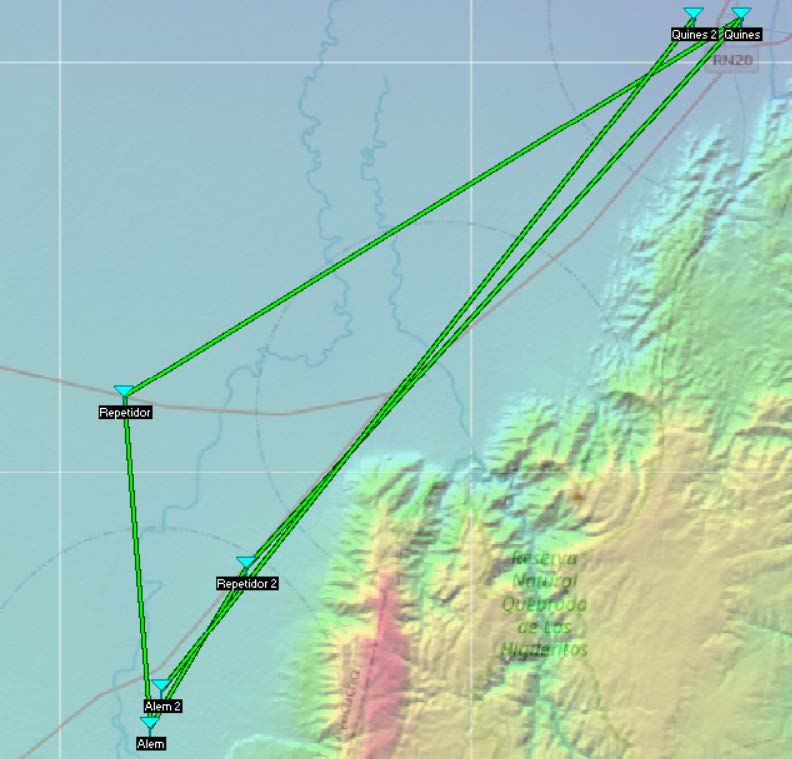
\includegraphics[width=\linewidth]{fotos_ema/imp_radio_mobile.jpg}
  \caption{implementación en Radio Mobile de los 3 enlaces.}
  \label{fig:enlaces_radiom}
\end{figure}
\clearpage
\subsubsection{Conexión directa}

En la Fig. \ref{fig:con_directa}, se presenta la conexión directa entre Leandro N. Alem y Quines.
La ventaja que presenta esta solución radica en el hecho de que se utilizan sólo dos transmisores, y 2 torres. El problema principal está en el hecho de que debido a la topografía del lugar, la altura necesaria para establecer la comunicación es mayor a las demás opciones, tal como se muestra en la tabla \ref{tab:altura_antenas}.

\begin{figure}[htbp]
  \centering
  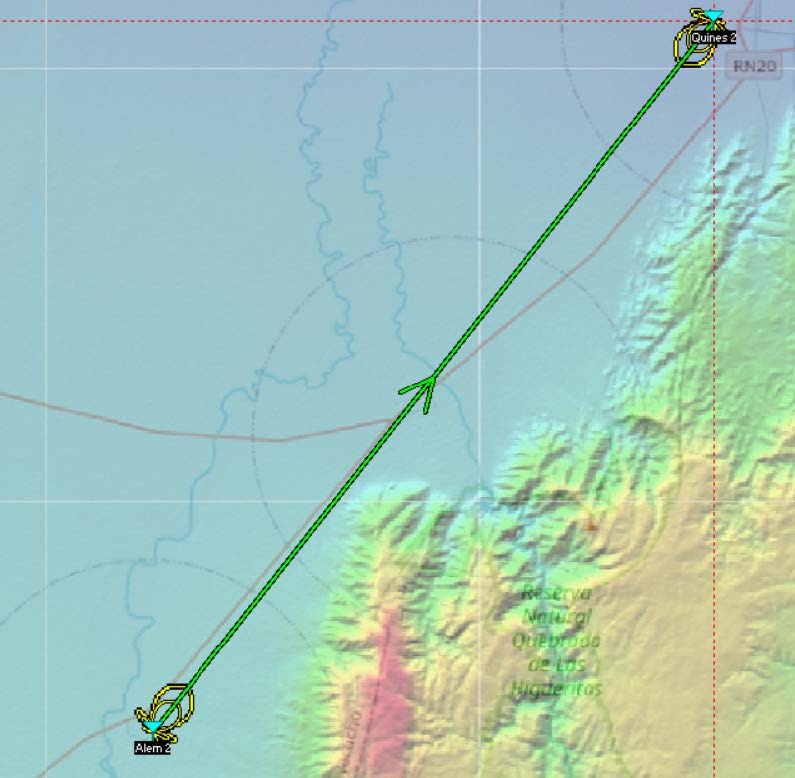
\includegraphics[width=0.55\linewidth]{fotos_ema/con_directa.jpg}
  \caption{conexión directa entre Leandro N. Alem y Quines.}
  \label{fig:con_directa}
\end{figure}
En la Fig. \ref{fig:sim_directa} se muestra el resultado de la simulación, demostrando con la misma el teorico funcionamiento del mismo.
\begin{figure}[htbp]
  \centering
  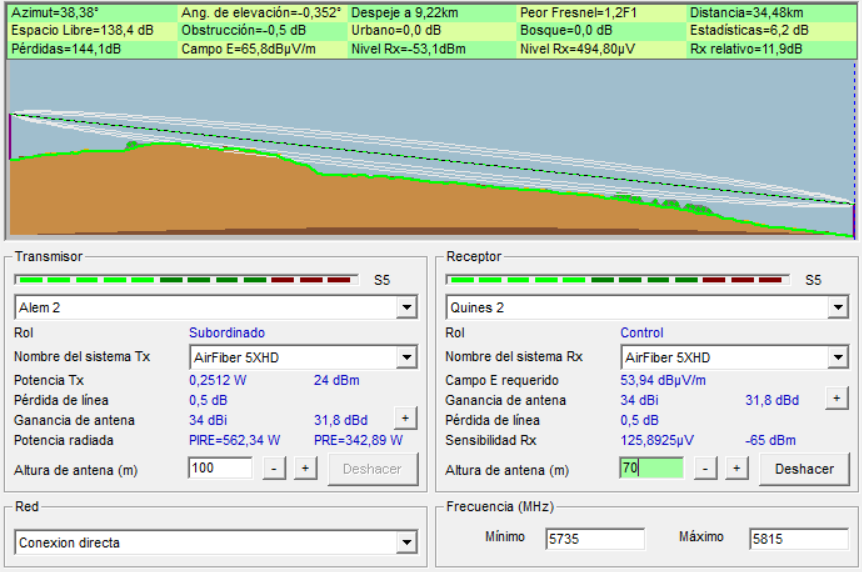
\includegraphics[width=0.7\linewidth]{fotos_ema/sim_directa.png}
  \caption{simulación de la conexión directa entre Leandro N. Alem y Quines.}
  \label{fig:sim_directa}
\end{figure}


En el trabajo práctico N$^{\text{o}}3$ se pueden analizar las simulaciones de los demás enlaces, así como el cálculo del presupuesto de potencia completo para el enlace directo\footnote{\href{https://docs.google.com/document/d/1dYO6yN0Ze9tsv_Ijca2n36-JYDfShurftSzc-x_Jx1I}{Trabajo Práctico N$^{o}$ 1 "Red troncal con radioenlace"}}, el cual verifica de manera analítica la viabilidad del enlace directo propuesto.


\subsubsection{Elección del tipo de enlace}
Observando los distintos enlaces propuestos, se decide optar por la conexión directa, ya que la misma presenta las siguientes ventajas:

\begin{itemize}
  \item  \textbf{Emplazamiento de 2 torres:} esta configuración necesita para su operación el emplazamiento de solamente 2 torres. 
  Si bien las opciones con repetidor necesitan torres de menor altura para su operación, el hecho de tener que armar una torre adicional, junto con 2 equipos, los cuales necesitan además supervisión técnica y mantenimiento, encarece en tal manera el sistema, que se justifica la utilización de solamente dos torres. 
  Aún más, el hecho de instalar una torre adicional, aunque sea de menor altura, deviene en mayores gastos administrativos, legales y técnicos, convirtiendo así a la conexión directa en la opción más asequible y sencilla.

  \item \textbf{ Menor mantenimiento:} debido a que solo se cuenta con 2 equipos, en lugar de 4, como lo es en el caso de las conexiones con repetidor, el mantenimiento de la instalación necesaria es menor.

  \item \textbf{ Mejor aprovechamiento del equipo a utilizar:} debido a los requerimientos de potencia y tasa de transferencia de bits, era necesario utilizar un equipo con las prestaciones previamente mencionadas, sin embargo, el equipo soporta conexiones de hasta 100 kilómetros de distancia. 
  Al colocar un repetidor en un radio cercano al emisor, se está desaprovechando esta capacidad, sobredimensionando el sistema, debido a que no existe un equipo que cubra menores distancias pero que cuente con las tasas de transferencia de bits necesarias.
\end{itemize}

\section{Red troncal con fibra óptica}

\subsection{Trayectoria y tipo de instalación que se realizará}



Un recorrido en línea recta entre ambas localidades sería el caso ideal y de menor distancia necesaria, pero implicaría una gran inversión en estructuras para poder transportar la fibra de forma aérea o en excavación en el caso que se haga de forma subterránea. 
Por lo tanto, debido al tipo de terreno montañoso que poseen los pueblos a unir, la conexión de fibra óptica se realizará de forma aérea usando el tendido de media tensión que une Quines y Leandro N. Alem, pasando por Luján.

La elección de usar el tendido eléctrico presenta un gran ahorro, ya que se utilizarán estructuras ya existentes. 
En las Fig. \ref{fig:tendido_media_tension_quines_lujan} y Fig. \ref{fig:tendido_media_tension_lujan_alem} se observa en verde el recorrido que realiza el tendido eléctrico de media tensión desde el centro de Quines hasta Luján y desde Luján hasta Leandro N. Alem, respectivamente.
Este análisis se realizó usando la herramienta Visor SIG \footnote{\href{https://sig.se.gob.ar/visor/visorsig.php?t=1}{Visor SIG}}.


\begin{figure}[ht!]
  \centering
  \subcaptionbox{tendido de media tensión desde Quines hasta Luján.\label{fig:tendido_media_tension_quines_lujan}}[.49\linewidth]{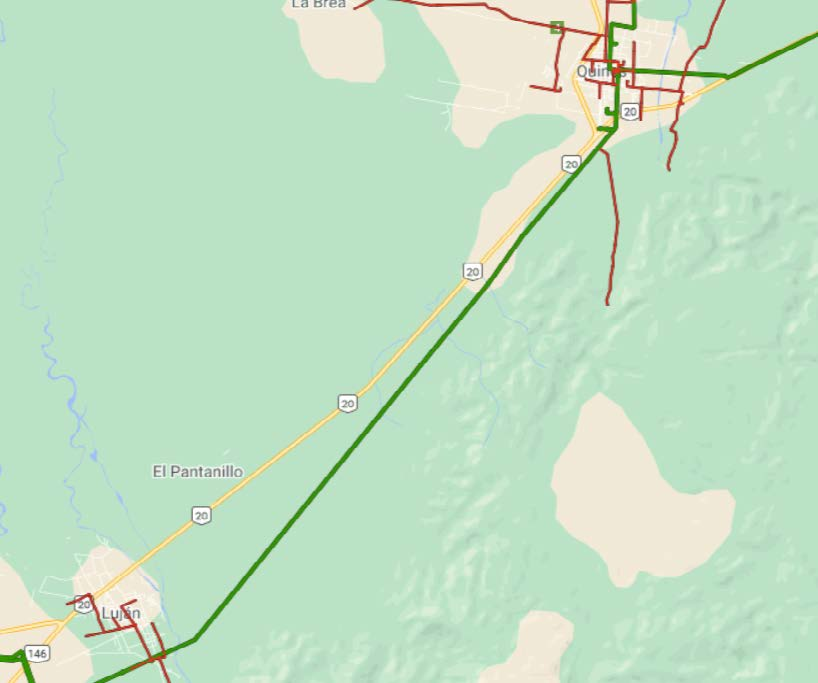
\includegraphics[height=11\baselineskip]{fotos_ema/tendido_media_tension_quines_lujan.jpg}}
  \hfill
  \subcaptionbox{tendido de media tensión desde Luján hasta Leandro N. Alem.\label{fig:tendido_media_tension_lujan_alem}}[.49\linewidth]{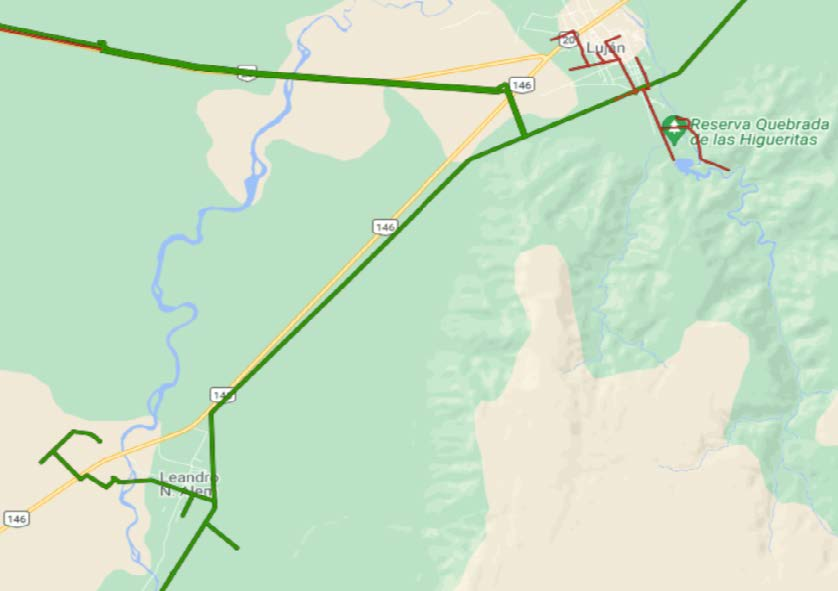
\includegraphics[height=11\baselineskip]{fotos_ema/tendido_media_tension_lujan_alem.jpg}}
  \caption{tendido de media tensión}
  \label{fig:tendido_media_tension}
\end{figure}


La Fig. \ref{fig:dist_quines_lujan_tendido_media_v} y Fig. \ref{fig:dist_quines_alem_tend_media_v} muestran las distancias que recorre el tendido eléctrico desde el centro de Quines hasta Luján y desde Quines hasta Leandro N. Alem, las cuales son 20556 Km y 37504 Km respectivamente. 

\begin{figure}[ht!]
  \centering
  \subcaptionbox{Distancia desde Quines hasta Luján por medio de tendido eléctrico de media tensión.\label{fig:dist_quines_lujan_tendido_media_v}}[.49\linewidth]{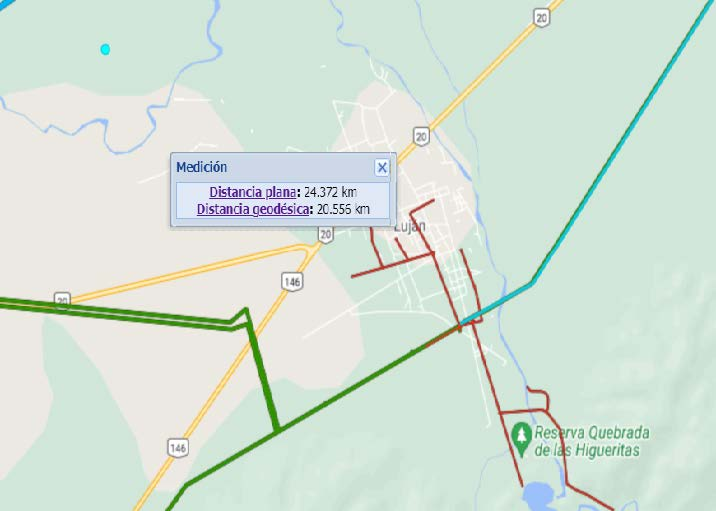
\includegraphics[height=11\baselineskip]{fotos_ema/dist_quines_lujan_tendido_media_v.jpg}}
  \hfill
  \subcaptionbox{Distancia desde Quines hasta Leandro N. Alem por medio de tendido eléctrico de media tensión.\label{fig:dist_quines_alem_tend_media_v}}[.49\linewidth]{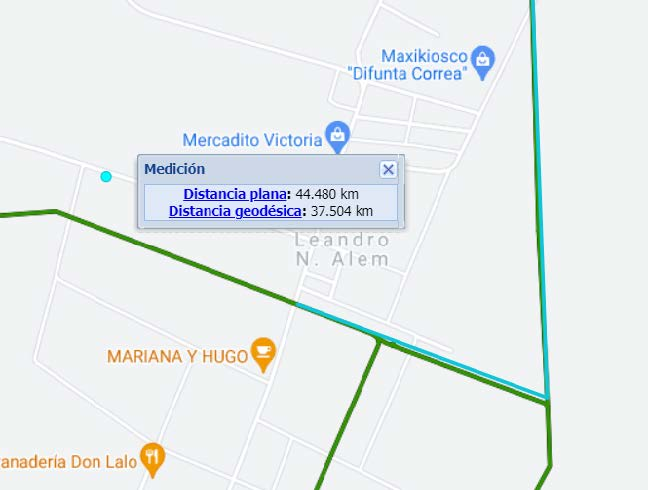
\includegraphics[height=11\baselineskip]{fotos_ema/dist_quines_alem_tend_media_v.jpg}}
  \caption{distancia teniendo en cuenta el tendido de media tensión}
  \label{fig:dist_tendido_media_tension}
\end{figure}



A la distancia final de 37504 Km que debe recorrer la fibra óptica para unir estas dos localidades se le debe sumar un 10\% para considerar los rollos de ganancia que se formarán en cada empalme\footnote{\href{https://www.teldor.com/files.php?actions=show&id=7655}{ADSS Installation Guide}} lo que da una distancia final de 41254 Km.

Otro medio que se puede usar para transportar la fibra óptica desde Quines hasta Leandro N. Alem, es a través del tendido de alta tensión que se ve en color rojo en la Figura 5.
Este camino se descarta, ya que se necesitan estructuras para llegar a Leandro N. Alem y el recorrido es mayor, por lo que se necesita mayor cantidad de fibra. 
Además, conseguir permiso para colocar fibra óptica en estos tendidos es algo muy costoso y difícil.

\begin{figure}[htbp]
  \centering
  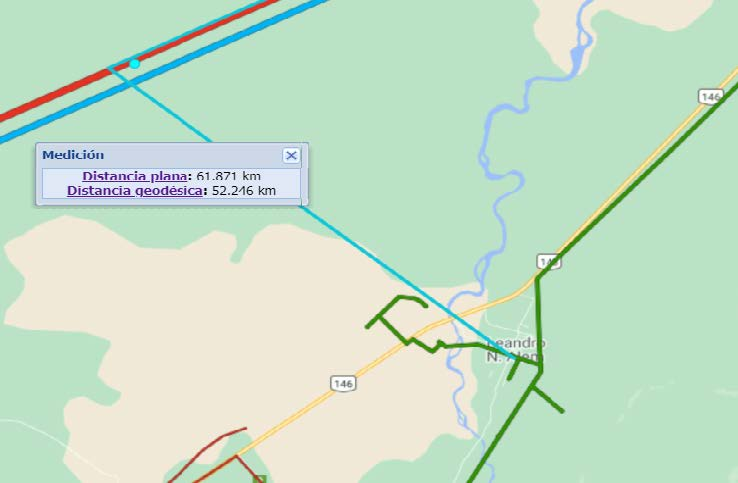
\includegraphics[width=0.5\linewidth]{fotos_ema/dist_quines_alem_tend_alta_v.jpg}
  \caption{distancia desde Quines hasta Leandro N. Alem por medio de tendido eléctrico de alta tensión.}
  \label{fig:dist_quines_alem_tend_alta_v}
\end{figure}

Se deben de tener en cuenta todas las medidas de seguridad debido a que se estará trabajando con postes que ya llevan un tendido eléctrico. 
Estos poseen una distancia de 80 metros entre sí aproximadamente. 
Primero se instalará el fiador entre vano y vano, el cual será una base para la instalación, seguidamente se colocará el guía cable y fijador al fiador los cuales facilitarán el tendido de la fibra en el vano. 
El artículo del sitio web Conectronica\footnote{\href{https://www.conectronica.com/fibra-optica/curso-fibra-optica/tipos-de-instalacion-de-fibra-optica}{Tipos de Instalación de Fibra óptica, Conectores}} ofrece los pasos recomendados a seguir en la instalación de fibra óptica de forma aérea.

\begin{figure}[htbp]
  \centering
  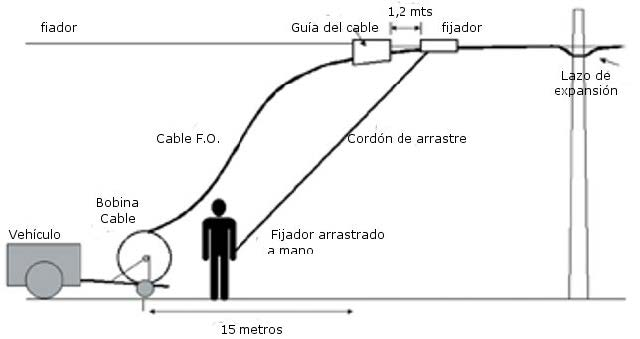
\includegraphics[width=0.7\linewidth]{fotos_ema/esq_inst_fo.jpg}
  \caption{esquema de instalación aérea de fibra óptica.}
  \label{fig:esq_inst_fo}
\end{figure}

El fiador deberá estar ajustado debidamente a un soporte A.D.S.S. \footnote{\href{https://www.preform.com.ar/tienda/telecomunicaciones/redes-de-fibra-adss/suspenciones/kit-retencion-adss-prolongador-grillete-y-preformado-120-mts/}{KIT SUSP ADSS MENSULA SUSPENSIÓN URBANA ( ARO Y ATADURA) ( HASTA 80 MTS)}} como el de la Fig. \ref{fig:soporte_adss} , ya que en él reposará el cable de fibra óptica. 

\begin{figure}[htbp]
  \centering
  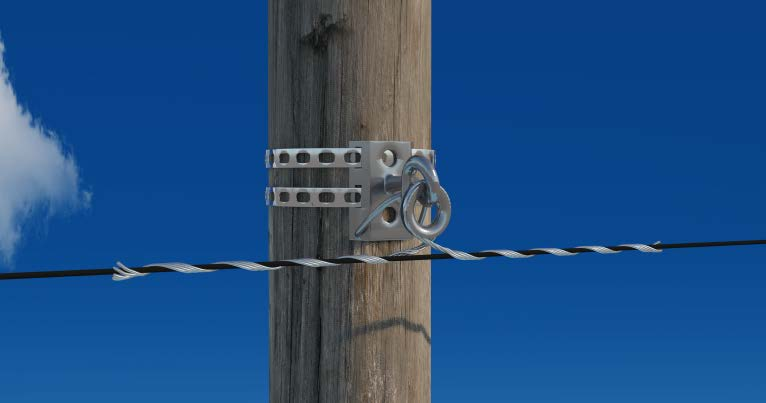
\includegraphics[width=0.7\linewidth]{fotos_ema/soporte_adss.jpg}
  \caption{Soporte A.D.S.S.}
  \label{fig:soporte_adss}
\end{figure}


A una distancia de 1,50 metros se colocarán dos abrazaderas, una de fijación y la otra que abrazará al cable propiamente dicho, dejando un radio de curvatura mínima de la fibra entre abrazaderas. Esto se puede observar en la Fig. \ref{fig:esq_col_abrazadera}.


\begin{figure}[htbp]
  \centering
  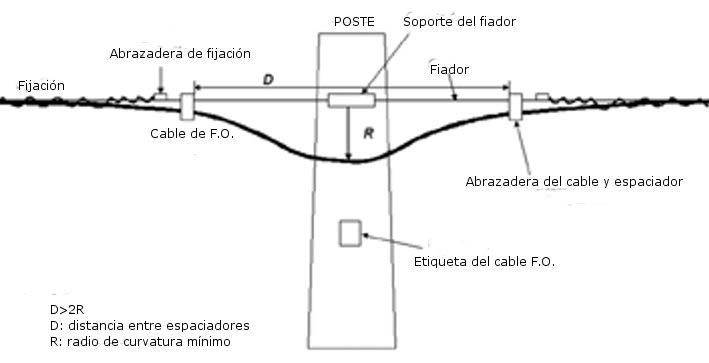
\includegraphics[width=0.7\linewidth]{fotos_ema/esq_col_abrazadera.jpg}
  \caption{Esquema de colocación de abrazaderas.}
  \label{fig:esq_col_abrazadera}
\end{figure}



%==================================================================================

En cuanto a la instalación, al momento del armado de ganancias se deberá usar una regleta tipo cruz\footnote{\href{https://articulo.mercadolibre.com.ar/MLA-909799496-cruz-de-reserva-100-x-100cm-galvanizada-para-fibra-optica-_JM?matt_tool=88481412&matt_word=&matt_source=google&matt_campaign_id=11618987428&matt_ad_group_id=113657532672&matt_match_type=&matt_network=g&matt_device=c&matt_creative=479785004862&matt_keyword=&matt_ad_position=&matt_ad_type=pla&matt_merchant_id=308510455&matt_product_id=MLA909799496&matt_product_partition_id=841218013617&matt_target_id=pla-841218013617&gclid=CjwKCAjw_JuGBhBkEiwA1xmbRUsQ-48g75U_LS2OkDkasr5E-iXwDYYjTvlZx3yOGCESphlHs3DjdhoC0lEQAvD_BwE }{Regleta tipo cruz}} como la de la Fig. \ref{fig:regleta_ruz}, la cual deberá tener un diámetro acorde a la curvatura máxima tolerable por la fibra para mantener la integridad del enlace.

\begin{figure}[htbp]
  \centering
  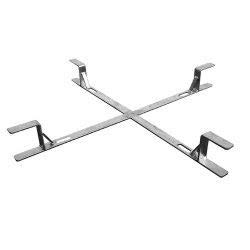
\includegraphics[width=0.4\linewidth]{fotos_ema/regleta_ruz.jpg}
  \caption{Regleta tipo cruz.}
  \label{fig:regleta_ruz}
\end{figure}


Al realizar un empalme se puede optar ya sea por caja de empalme estaca como la mostrada en la Figura \ref{fig:caja_empalme} o cierres de empalme como se muestran en la Fig. \ref{fig:cierres_empalma}.


\begin{figure}[ht!]
  \centering
  \subcaptionbox{Caja de empalme estaca.\label{fig:caja_empalme}}[.49\linewidth]{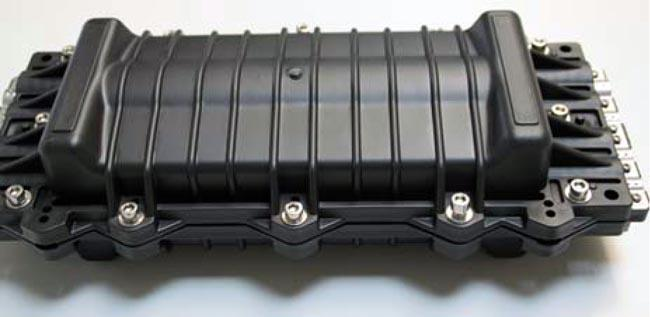
\includegraphics[height=7\baselineskip]{fotos_ema/caja_empalme.jpg}}
  \hfill
  \subcaptionbox{Cierres de empalme.\label{fig:cierres_empalma}}[.49\linewidth]{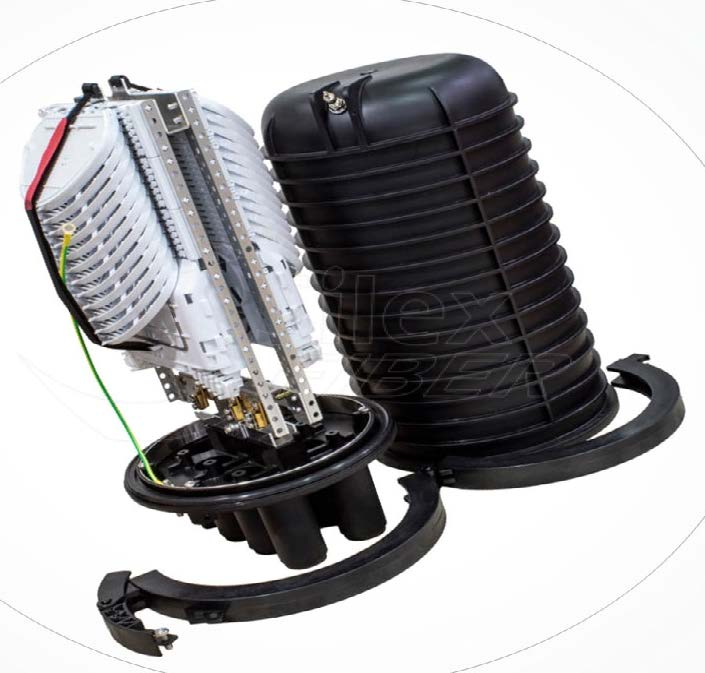
\includegraphics[height=7\baselineskip]{fotos_ema/cierres_empalma.jpg}}
  \caption{Opciones de empalme}
  \label{fig:opciones_empalme}
\end{figure}


Los dos puntos anteriores de la instalación quedan ilustrados en la Fig. \ref{fig:inst_gan_emp_fo}.


\begin{figure}[htbp]
  \centering
  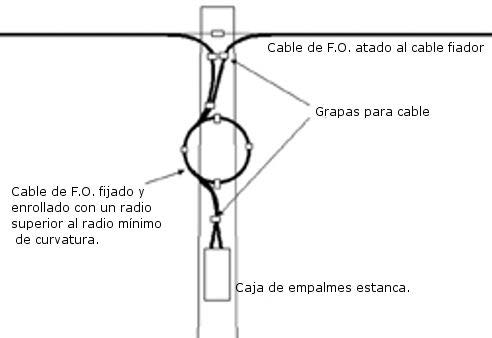
\includegraphics[width=0.35\linewidth]{fotos_ema/inst_gan_emp_fo.jpg}
  \caption{Instalación de ganancia y empalme de fibra óptica.}
  \label{fig:inst_gan_emp_fo}
\end{figure}
 
%==================================================================================
\subsection{Determinación del tipo de cable de fibra óptica}

Teniendo en cuenta las largas distancias que se desean cubrir es que se opta por elegir una fibra óptica monomodo, ya que permite cubrir trayectos mayores a 10 km, manteniendo altas velocidades de transmisión de datos. 
Por otro lado, debido a que se transportará el cable utilizando las instalaciones de media tensión, es necesario que el cable sea del tipo A.D.S.S., lo cual significa que es autosoportado y totalmente dieléctrico. 
Esto brinda seguridad a la instalación y posterior mantenimiento tanto del tendido eléctrico como del tendido de la fibra. 

En el trabajo práctico N$^{\text{o}}$ 4  se analizan 3 tipos de cables, cada uno posee un tipo de fibra que se corresponde con las distintas normas de la UIT-T\footnote{\href{https://docs.google.com/document/d/1yDd0ZPVQQ6xVwB_qNpXz09s-V0TPoRrC3KIsim4-Geg/edit}{Trabajo Práctico N$^{\text{o}}$ 4 "Red de Troncal con Fibra Óptica"}}. A continuación, se muestra en la tabla \ref{tab:fo_options}, una comparativa con las distintas características físicas que brindan las hojas técnicas de los distintos modelos:

\begin{table}[htbp]
  \centering
\begin{tabular}{|c|c|c|c|} \hline 
\textbf{Características} & \textbf{Opción 1} & \textbf{Opción 2} & \textbf{Opción 3} \\ 
\hline 
\textbf{Marca} & Optral \tablefootnote{\href{https://fibromarket.com/fichas/cables/cable_antirroedor-de-fibra-de-vidrio-optral-sm.pdf}{Opción 1}} & GLC & Cablena \\ 
\hline 
\textbf{Modelo} & - & GLCADSS80-6/12 \tablefootnote{\href{https://glctec.com/wp-content/uploads/2022/01/catalogo_2022-1.pdf}{Opción 2, página 29}} & ETP-FO-003\tablefootnote{\href{https://fibromarket.com/fichas/cables/cable_adss_12_fo_etp-fo-003_-_asu_cablena-fibromarket.pdf}{Opción 3}} \\ \hline 
\textbf{Largo por bobina} & 4,2 km & 4 km & - \\ 
\hline 
\textbf{Norma} & G.652.B & G.652.D & G.655 \\ 
\hline 
\textbf{Cantidad de pelos} & 6 & 6/12 & 12 \\ 
\hline 
\textbf{Distancia entre vanos} & - & 80 m & 80 m \\ 
\hline 
\end{tabular}
\caption{opciones de cables de fibra óptica.}
\label{tab:fo_options}
\end{table}

Teniendo en cuenta lo analizado, las fibras que se corresponden con la norma G.655, se encuentran optimizadas para trabajar con señales en la banda de 1550 nm.
Esto conlleva un problema a la hora de elegir los equipos transceptores debido a que generalmente se utilizan distintas bandas para una transmisión bidireccional en un solo cable, mientras que este tipo de fibra cuenta con un rango muy escaso de operación, resultando en mayores costos al necesitar dos pelos, uno para la trasmisión y otro para la recepción.

Para poder decidir sobre las dos opciones restantes será necesario obtener más información sobre los equipos transceptores y en qué frecuencias pueden operar, debido a que la fibra óptica que se corresponde con la norma G.652.B posee un pico de agua que limita las bandas que puede utilizar el equipo.

%=================================================================================

\subsection{Determinación de los equipos}

\subsubsection{Switches}

Para la implementación de la comunicación, se presentan en el práctico 3 equipos de switches que serán los que coordinen la transmisión y recepción de datos, uno de la marca Cisco y otros 2 de la marca Ubiquiti. 

Del análisis de los equipos se determina que el equipo más completo es la opción 3, siendo el switch de la marca Ubiquiti modelo ES 48 LITE EdgeSwitch, ya que admite los 3 tipos de conectores utilizados en la transmisión de datos, ethernet, SFP y SFP+. 
Además, este presenta la mayor cantidad de puertos Ethernet, los cuales jugarán un rol importante a la hora de distribuir los datos a los distintos clientes. 
Como desventaja, este equipo presenta el mayor consumo de los 3, pero debido a la cantidad de puertos y su bajo precio, se considera esta desventaja como insignificante. 

\subsubsection{Transceptores}

Teniendo en cuenta los puertos presentes en el switch seleccionado, se procede a buscar los módulos SFP y SFP+ que permitirán la comunicación a través de la fibra óptica.  
Del análisis realizado en el trabajo práctico N$^\text{{o}}$ 3, para no incurrir en mayores gastos, se elige la opción 1 para realizar un posterior cálculo del enlace, ya que a pesar de que hay que importarla, es económica. 
Este es el módulo SFP bidireccional de la marca FS, modelo SFP-GE-BX80, el cual soporta distancias de hasta 80 kilómetros.

%==============================================================================

Debido a las velocidades de transmisión que presenta el equipo elegido previamente y la tasa de transferencia necesaria para este proyecto, es que basta con la utilización de 1 pelo de fibra óptica para cumplir los requerimientos. 
Teniendo en cuenta las longitudes de onda que se utilizan en ambos tipos de fibra y la recomendación del fabricante, ambos cables son compatibles con este dispositivo, ya que el mismo no opera en la banda E. 
Más aún, las atenuaciones y las pérdidas para las bandas utilizadas, S y C, son las mismas en ambos tipos de fibra\footnote{\href{https://www.belden.com/blogs/reusing-singlemode-fiber-here-s-what-the-g-652d-and-g-657a1-standards-have-to-say\ }{G652D and G 657A1 standards}}.


\subsection{Propuestas de enlace}

En el trabajo práctico se presentaron y analizaron dos alternativas de enlaces. 
A continuación se muestran los esquemas de conexión para cada uno de ellos.

\subsubsection{Enlace directo}
\label{section:enl_dir}

En la Fig. \ref{fig:esq_enl_directo}, se observa un esquema de la conexión, mostrando empalmes, conectores y equipos utilizados en la implementación del enlace. 
Esto permite brindar una idea más gráfica del enlace, lo cual será útil para posteriores cálculos tanto económicos como técnicos.


\begin{figure}[htbp]
  \centering
  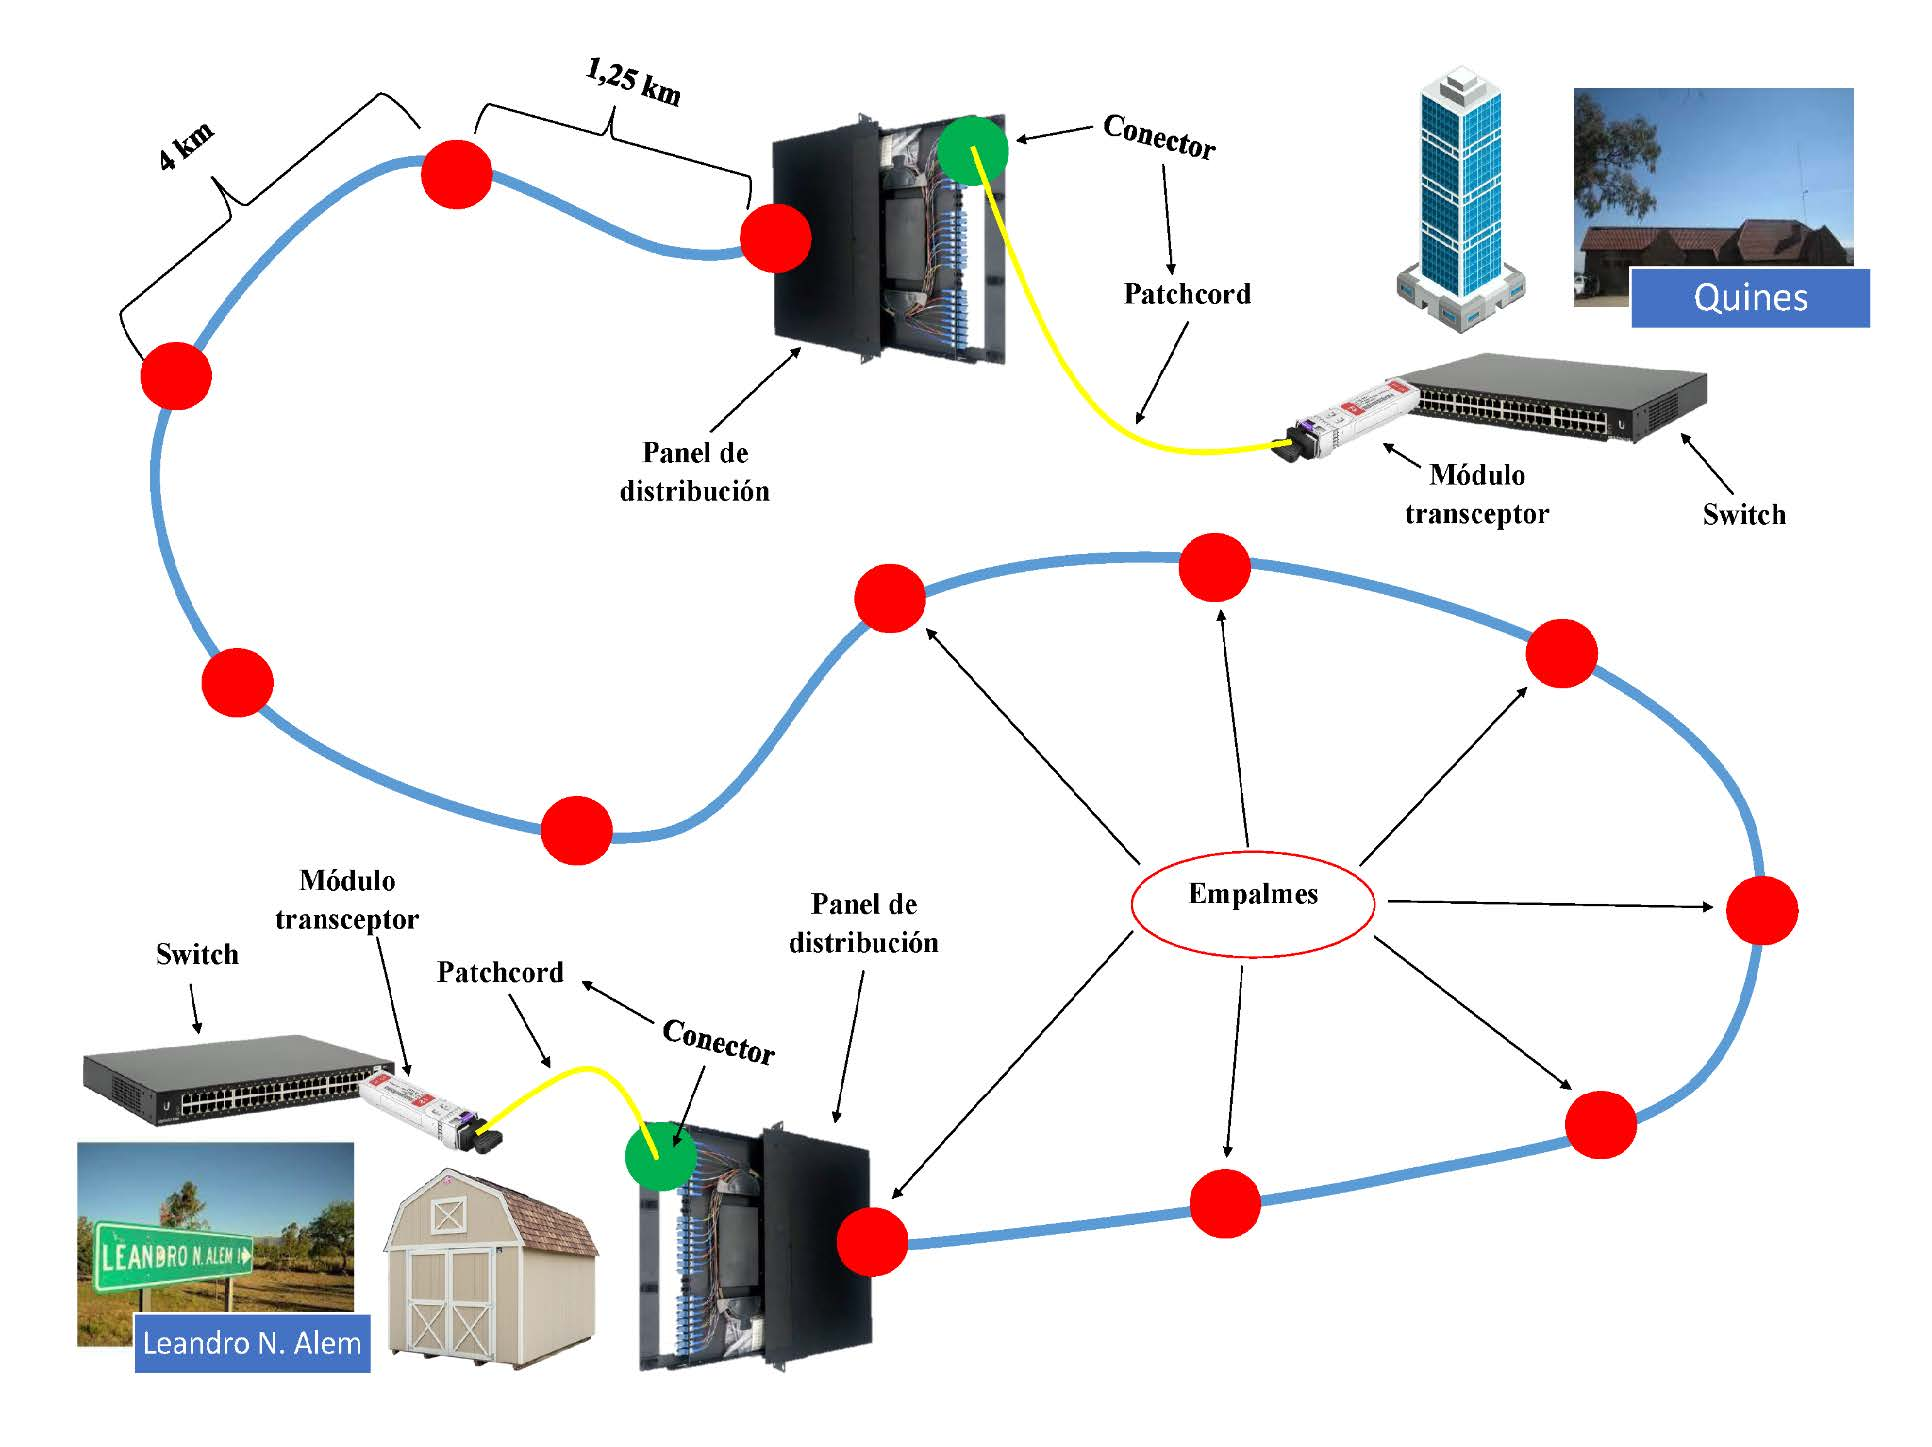
\includegraphics[width=0.7\linewidth]{fotos_ema/esq_enl_directo.jpg}
  \caption{Esquema del enlace.}
  \label{fig:esq_enl_directo}
\end{figure}


Los resultados de los análisis realizados indican que el enlace es viable, incluso si la potencia utilizada es la mínima. 
Aún más, se respeta el margen mayor a 5 dB previamente indicado, lo cual brinda mayor certeza en la viabilidad de la instalación.

 \subsubsection{Enlace alternativo}

Se propone colocar una estación repetidora en la localidad de Luján. 
Esto con el objetivo de incluir a Luján como posible zona comercial, y además brindar una alternativa a la instalación en el caso de que no se cuente con la posibilidad de importar el módulo de la opción 1, el presupuesto no sea lo suficientemente alto como para adquirir el módulo de la opción 4, o no se consiga stock de los mismos, dejando como opción disponible la opción 3, de la cual existen alternativas en el mismo margen de precio\footnote{\ $  $Alternativas\ }. 
Para esto se utilizará el mismo switch que se seleccionó previamente, el cual como posee 2 entradas SFP, es posible usar una entrada para el tramo Quines-Luján y otra para el tramo Luján-Leandro N. Alem. 
Teniendo en cuenta que la distancia calculada entre Quines y Luján es de 20,55 Km y la distancia entre Luján y Leandro N. Alem es de 16,95 Km, se procede a calcular nuevamente los enlaces, esta vez por tramos. 
Los datos son los mismos que los mostrados previamente, variando la distancia en kilómetros, la cantidad de empalmes y conectores utilizados. 

Se considera una distancia  de 22,65 km para el tramo Quines-Luján, y una distancia de 18,65 km para el tramo Luján-Leandro N. Alem. 
Se considerarán 8 conectores, 2 en Leandro N. Alem, 2 en Quines y 4 en Luján. Además se tienen 13 empalmes, 7 empalmes entre Quines y Luján y 6 empalmes entre Luján y Leandro N. Alem. 
En la Figura 15 se muestra un esquema de la conexión representando los empalmes, los equipos y las localidades presentes. 


\begin{figure}[htbp]
  \centering
  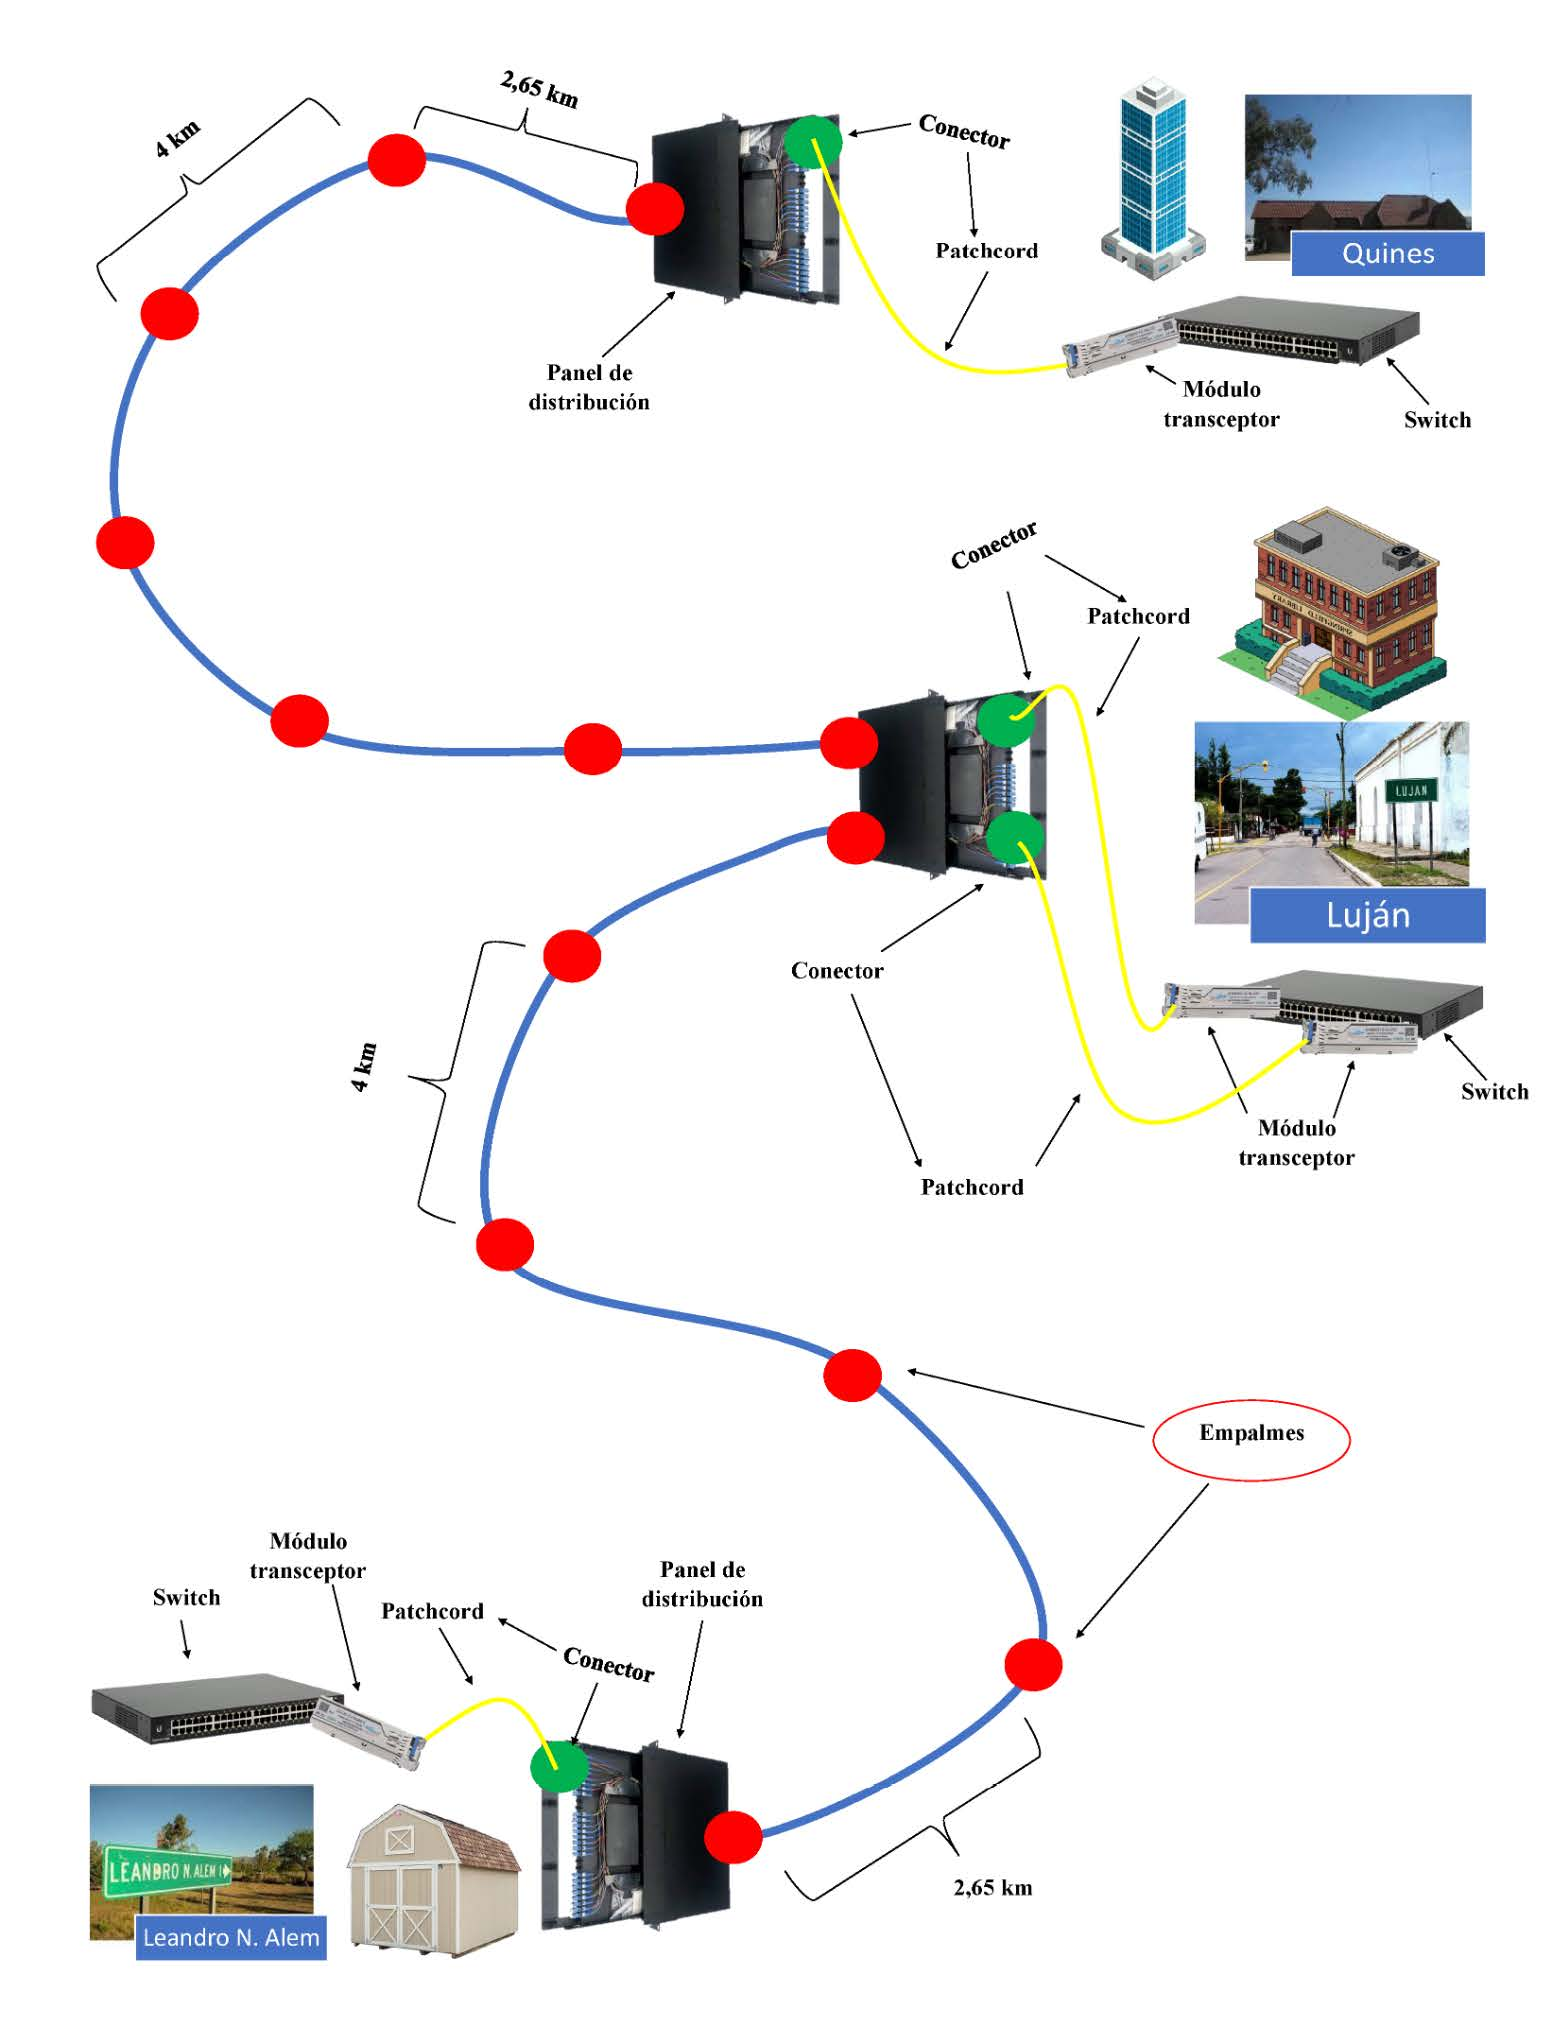
\includegraphics[width=0.7\linewidth]{fotos_ema/esq_enl_lujan.jpg}
  \caption{Esquema de conexión alternativa.}
  \label{fig:esq_enlace_lujan}
\end{figure}


\paragraph{Tramo Quines-Luján:}


Se observa como resultado que el enlace es viable tanto para la mínima como para la máxima potencia que ofrece el módulo, debido a que se respeta incluso el margen de 5 dB que se elige como referencia de posibles errores adicionales de instalación y/o imperfecciones en la fibra.

\paragraph{Tramo Luján-Leandro N. Alem}

Se muestra en la tabla \ref{tab:enl_lujan_alem} el cálculo del enlace. Se considera un $N_2$igual a 0,32 debido a que existen 6 empalmes en 18,65 Km, dando como resultado dicho número. 


Se observa como resultado que el enlace es viable tanto para la mínima como para la máxima potencia que ofrece el módulo, debido a que se respeta incluso el margen de 5 dB que se elige como referencia de posibles errores adicionales de instalación y/o imperfecciones en la fibra. 
Es por ello que con la decisión de colocar una estación repetidora en Luján, es posible obtener 2 opciones de enlaces viables que aseguren la comunicación entre los equipos.

\subsubsection{Conclusión}

Como se demostró en la sección \ref{section:enl_dir}, el enlace de fibra óptica es viable desde Quines hasta Leandro L. Alem sin necesidad de hacer uso de un repetidor o amplificador. 
De igual manera, el uso de un repetidor en la localidad de Luján abre las puertas a expandir la cantidad de posibles clientes en un futuro y permitir así una fácil amortización de la inversión.


\clearpage
\part{Red de acceso}

\section{Red de acceso con radioenlace}

\subsection{Determinación de la tasa de transferencia necesaria y cálculo de los accesos}

Del estudio socioeconómico realizado sobre la localidad de Leandro N. Alem se obtuvo que 83 hogares del total de la población serán potenciales clientes del servicio brindado. 
También se obtuvo como conclusión que 25 clientes optarán por el pack básico, 44 clientes utilizarán el pack intermedio y 14 clientes el pack premium. 
En la Tabla~1 se observa un resumen de los valores más importantes a tener en cuenta.


\begin{table}[htbp]
  \resizebox*{\textwidth}{!}{
  \centering
  \begin{tabular}{|c|p{0.2\linewidth}|p{0.2\linewidth}|p{0.2\linewidth}|p{0.2\linewidth}|} 
  \hline 
  \textbf{Servicio} & \textbf{Tasa de datos} & \textbf{Pack básico} & \textbf{Pack intermedio} & \textbf{Pack premium} \\ \hline 
\textbf{Canal SDTV} & 1.5 Mbps & 50 canales & 50 canales & 50 canales \\ \hline 
\textbf{Canal HDTV} & 6 Mbps & - & - & 6 canales \\ \hline 
\textbf{VoIP\footnote{ La tasa de datos es despreciable a la hora de realizar los cálculos.}} & 30 kbps & 30 kbps & 30 kbps & 30 kbps \\ \hline 
\textbf{Internet} & - & - & 6 Mbps & 15 Mbps \\ \hline 
\textbf{Clientes} & - & 25 & 44 & 14 \\ \hline 
\end{tabular}}%
\caption{contenido de pack de servicios.}
\label{tab:cont_pack_servicio}
\end{table}
 



 Según el Ministerio de Planificación Federal, Inversión Pública y Servicios, en el año 2.009, en la República Argentina había aproximadamente 10 millones de hogares y cerca de 12 millones de televisores\footnote{\href{http://www.infoleg.gob.ar/basehome/actos_gobierno/actosdegobierno14-9-2009-2.htm}{Televisores por hogar}}. 
 Se estima entonces que la cantidad de televisores supera en un 20\% la cantidad de hogares. 
 Este porcentaje no se distribuye uniformemente sobre la población, varía según el poder adquisitivo de las personas y por consiguiente lo hace sobre los clientes, siendo más frecuente que una persona con un buen sueldo tenga más de un televisor. 
 Por lo tanto, se puede decir que el 20\% de los 83 potenciales clientes, que corresponde a 17 clientes, tienen 2 televisores.
Si se considera un máximo de 2 televisores por hogar y el poder adquisitivo de cada grupo, se estima que 8 clientes correspondientes al pack premium cuentan con dos televisores, 6 clientes en el pack intermedio y 3 en el pack básico.
El resto de los clientes solo cuentan con un televisor. 
Además, se considera que los clientes pertenecientes a los pack intermedios y premium hacen uso del 60\% de los megas correspondientes a cada pack.

La tasa de transferencia en el peor de los casos para el pack premium da como resultado 18,42 Mbps, como muestra la ecuación \ref{eq:tasa_transf_premium}. 
Esto se calcula de suponer que 8 clientes de los 14 (57\%) usan 2 canales HD simultáneamente, 6 clientes (43\%) utilizan solo un canal HD, sumando además el un factor de simultaneidad del 60\% en el internet. 


\begin{equation}
  2*6*{10}^6*0.57+6*{10}^6*0.43+0.6*15*{10}^6=18.42 \text{ Mbps}
  \label{eq:tasa_transf_premium}
\end{equation}


De forma similar se realizaron los cálculos para los pack intermedios y básicos. 
Los resultados se muestran en la ecuación \ref{eq:tasa_transf_int} y ecuación \ref{eq:tasa_transf_basic} respectivamente. 


\begin{equation}
 2*1.5*{10}^6*0.136+1.5*{10}^6*0.863+ 0.6*6*{10}^6=5,3 \text{Mbps} 
 \label{eq:tasa_transf_int}
\end{equation}

\begin{equation}
 2*1.5*{10}^6*0.12+1.5*{10}^6*0.88=1,68 \text{ Mbps}
 \label{eq:tasa_transf_basic}
\end{equation}
 

 En la Fig. \ref{fig:cuadrantes_alem} se puede observar en rojo los cuadrantes en los cuales se concentra mayor cantidad de gente y con un icono verde la ubicación de las antenas de la Autopista de la Información. 
 Observando el tamaño de los hogares, se supone que los grupos con mayor poder adquisitivo se encuentran entre los cuadrantes que van del 1 al 6, los cuales pueden ser potenciales clientes de los packs intermedio y premium. 
 Sin embargo, entre los cuadrantes 1 y 2 se encuentra una antena Wi-Fi (5 GHz) brindando internet gratis por parte del gobierno. 
 Considerando esto se decidió tener prioridad en los cuadrantes 3, 4, 5 y 6 a la hora de decidir la ubicación del Access Point (AP). Por otra parte, los cuadrantes del 11 al 14 no se ven alcanzados por ninguna antenas del gobierno, por lo que se estima que brindando un servicio que antes no disponían se encontrarán potenciales clientes en esta zona. 
 Por último está la zona céntrica donde se encuentra la plaza, en los cuadrantes 9 y 10. Esta zona cuenta con una antena Wi-Fi (2,4 GHz) pero la misma se encuentra saturada, rondando en promedio los 45 clientes\footnote{\href{http://wifi.sanluis.gov.ar/}{Antenas Wi-Fi de la provincia de San Luis}}.


\begin{figure}[htbp]
  \centering
  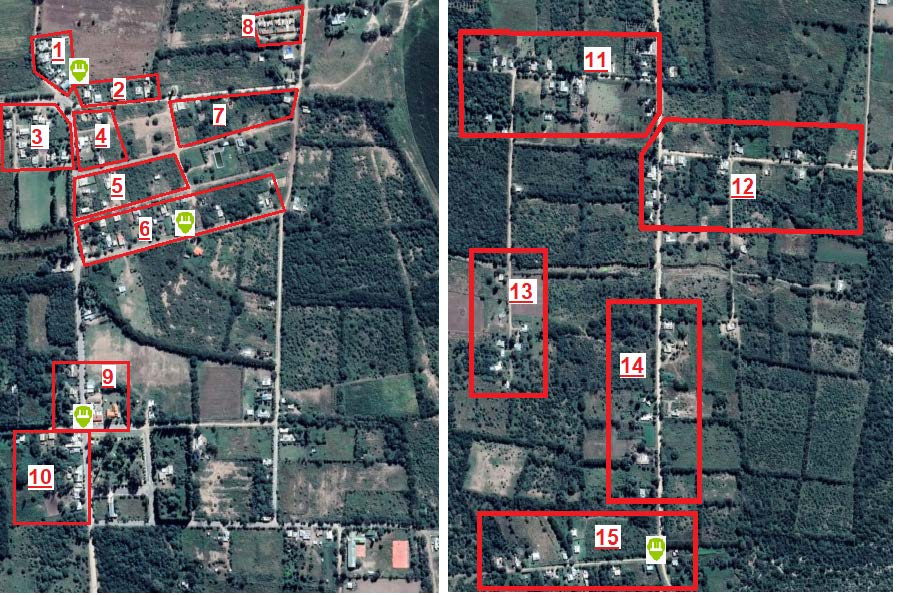
\includegraphics[width=0.8\linewidth]{fotos_ema/cuadrantes_alem.jpg}
  \caption{a la izquierda la zona norte y a la derecha la zona sur de la localidad de leandro N. Alem.}
  \label{fig:cuadrantes_alem}
\end{figure}

La cantidad de AP que se utilizarán para lograr la mayor cobertura posible y brindarle el servicio a los clientes se calcula a partir de la tasa de transferencia requerida por cliente teniendo en cuenta el peor de los casos.
Para el siguiente cálculo se optó por no considerar el pack básico, de esta forma se sobredimensiona el sistema para un futuro crecimiento en caso de que nuevos clientes quieran adquirir el servicio y/o aquellos que quieran adquirir un mejor pack. 
El promedio entre el caso más desfavorable de los pack intermedio y premium da como resultado 11,86 Mbps como se observa en la ecuación \ref{eq:prom_desf}. 

\begin{equation}
  \frac{18.426*{10}^6+5.3*{10}^6}{2}=11.86 \text{ Mbps}
  \label{eq:prom_desf}
\end{equation}

La tasa de transferencia total para brindar el servicio viene dada por el valor de la Ecuación \ref{eq:prom_desf} multiplicada por cantidad de clientes. Esto se ve reflejado en la ecuación \ref{eq:total_mbps_need}:

\begin{equation}
  83 * 11.86*{10}^6 = 984.38 \text{ Mbps}
  \label{eq:total_mbps_need}
\end{equation}

de los cuales se estima que por la cantidad de casas que se observan en la figura \ref{fig:cuadrantes_alem}, el 80 \% de la población vive en los cuadrantes del 1 al 9 y el 20\% restante se encuentra distribuido entre los cuadrantes 10 al 15. 
Teniendo en cuenta esta distribución de la población, se utilizarán AP que trabajen en la banda de 2,4 GHz y 5 GHz, de esta forma los clientes que se encuentran distribuidos en los extremos de la localidad serán alcanzados por las antenas de 2,4 GHz ya que estas cuentan con mayor alcance a costas de menor transferencia de bits. 
Por otro lado, en las partes que concentran mayor cantidad de clientes se utilizarán AP que trabajen en 5 GHz brindando una mayor tasa de transferencia pero menor alcance.

Hay que considerar que las antenas elegidas deben tener una tasa bruta de el doble de la tasa de transferencia calculada en la ecuación \ref{eq:total_mbps_need} ya que se pierde alrededor del 50\% de la capacidad de transmisión para garantizar que  la información se transmite de forma segura. 
Siendo así, la tasa de transferencia total es de 1.968 Mbps. 
Sin embargo, esta tasa de transferencia se distribuye entre los equipos cuando la cantidad de APs utilizadas aumenta y no es necesario que un solo equipo soporte el total. 

\subsection{Elección de los puntos de acceso}

La elección de los AP se basó en la tasa de transferencia necesaria calculada en el punto anterior. 
A continuación en la tabla \ref{tab:carac_ap} se muestran las características de los dos equipos AP que se analizaron: Aruba AP-375 y Altai A3-Ei.

En la tabla se observa la potencia del transmisor y la sensibilidad de recepción de los equipos, además de su familia de protocolos, tipo de antena y tasa de transferencia. 
Tanto la potencia del transmisor, como la sensibilidad del receptor, poseen un rango de valores que varía dependiendo el tipo de modulación elegida.


\begin{table}[htbp]
  \resizebox*{\textwidth}{!}{
\centering
\begin{tabular}{|c|p{0.1\textwidth}|p{0.2\textwidth}|p{0.2\textwidth}|p{0.2\textwidth}|p{
0.2\textwidth}|p{0.1\textwidth}|} 
\hline 
\textbf{Modelo de antena}&\textbf{Banda de frecuencia} & \textbf{Tasa de transmisión} & \textbf{Antena} & \textbf{Rango potencia transmisor} & \textbf{Rango sensibilidad receptor} & \textbf{Familia protocolos} \\ 
\hline 
\multirow{ 2}{*}{Aruba AP-375\tablefootnote{\href{https://www.arubanetworks.com/assets/ds/DS_AP370Series.pdf}{Datasheet Aruba AP-375}}}&2,4 GHz & Hasta 300 Mbps & 2x2 MIMO\newline omnidireccional  & Max: 23 dBm\newline Min: 18 dBm & Min: -93 dBm\newline Max: -71 dBm & 802.11n \\ 
\cline{2-7}
&5 GHz & 1733 Mbps & 4x4 MU-MIMO\newline omnidireccional & Max: 22 dBm\newline Min: 15 dBm & Min: -87 dBm\newline Max: -61 dBm & 802.11ac \\ 
\hline 
\multirow{ 2}{*}{Altai A3-Ei\tablefootnote{\href{https://www.altaitechnologies.com/portfolio-item/a3-ei/}{Datasheet Altai A3-Ei}}} &2,4 GHz & Hasta 450 MBps & 3x3:3 MIMO & Max:30 dBm \newline Min: 25 dBm & HT20: -92dBm \newline HT40: -88dBm & 802.11n \\ 
\cline{2-7}
&5 GHz & Hasta 1300 MBps & 3x3:3 MIMO & Max:30 dBm \newline Min: 25 dBm & HT20: -92dBm \newline HT40: -88dBm & 802.11ac \\ 
\hline
\end{tabular}}
\caption{características de los puntos de accesos considerados.}
\label{tab:carac_ap}
\end{table}

Mediante la tabla \ref{tab:carac_ap}  y los datasheet de cada uno de los AP, se puede observar que las especificaciones técnicas de los dos equipos son muy similares pero la ventaja y la razón por la cual se optó por usar el AP Aruba AP-375 es debido a que su antena es omnidireccional, lo cual no ocurre en el AP Altai A3-Ei que posee una antena direccional. 
Como los AP se colocarán en zonas céntricas de la ciudad, se necesita que posean antenas omnidireccionales para abarcar todos los alrededores. 
Además, este tipo de AP es el usado por la autopista de la información para ofrecer  Wi-Fi gratuito del gobierno lo que nos asegura su facilidad de adquisición de repuestos. 
La conexión desde el nodo hasta el POE será realizada por fibra óptica por medio de un transceptor SFP. Para poder acoplarse se necesitará un adaptador fibra-Ethernet.

\subsection{Elección del Equipo Local del Cliente}

El próximo equipo a elegir son los CPE (Equipo Local del Cliente) que se instalarán en los domicilios de los clientes para conectarse a los AP. 
De igual manera que en el análisis de selección de AP, se analizan los equipos para las dos diferentes frecuencias de trabajo. 
En las siguientes tablas se detallan los dispositivos elegidos junto a sus alternativas:

\subsubsection{Para 5 GHz/ 2,4 GHz}

En la tabla \ref{tab:carac_CPE_5} se muestran las características de las 2 opciones consideradas para este proyecto.
Las opciones son la antena Mikrotik LHG 5 AC \footnote{\href{https://mikrotik.com/product/lhg_5_ac}{Datasheet Mikrotik LHG 5 ac}} y la antena TP-Link CPE 710 \footnote{\href{https://static.tp-link.com/2020/202003/20200324/CPE\%20series-Datasheet.pdf}{Datasheet TP-Link CPE 710}}.


\begin{table}[htbp]
  \resizebox*{\textwidth}{!}{
  \centering
    \begin{tabular}{|c|c|c|c|c|c|c|}
\cline{2-7}    \multicolumn{1}{r|}{} & Modelo & Velocidad (5 GHz/2.4 GHz) & Protocolos & Potencia de transmisión & Sensibilidad & Ganancia de antena \\
    \hline
    \multirow{2}[4]{*}{Elegida} & \multirow{2}[4]{*}{Mikrotik-LHG 5} & 867 Mbps  & \multirow{2}[4]{*}{802.11a/n/ac} & \multirow{2}[4]{*}{Hasta 25 dBm} & \multirow{2}[4]{*}{Hasta -96 dBm} & \multirow{2}[4]{*}{24,5 dBi} \bigstrut\\
\cline{3-3}         &      & No posee &      &      &      &  \bigstrut\\
    \hline
    \multirow{2}[4]{*}{Alternativa} & \multirow{2}[4]{*}{TP-link-CPE 710} & 867 Mbps & \multirow{2}[4]{*}{802.11a/n/ac} & \multirow{2}[4]{*}{Hasta 27 dBm} & \multirow{2}[4]{*}{Hasta -93 dBm} & \multirow{2}[4]{*}{23 dBi}\bigstrut\\
\cline{3-3}         &      & 300 Mbps &      &      &      &  \bigstrut\\
    \hline
    \end{tabular}}%
    \caption{características de CPE para 5 GHz/ 2.4 GHz.}
  \label{tab:carac_CPE_5}%
\end{table}%


\subsubsection{Para 2,4 GHz}
En la tabla \ref{tab:carac_CPE_24} se muestran las características de las 2 opciones consideradas para este proyecto para la conexión utilizando la frecuencia de 2,4 GHz.

% Table generated by Excel2LaTeX from sheet 'page-1_table-1'
\begin{table}[htbp]
  \resizebox*{\textwidth}{!}{
  \centering
    \begin{tabular}{|c|c|c|c|c|c|c|}
\cline{2-7}    \multicolumn{1}{r|}{} & Modelo & Velocidad (2.4 GHz) & Protocolos & Potencia de transmisión & Sensibilidad & Ganancia \\
    \hline
    Elegida & TP-link CPE220 V3.0 \tablefootnote{\href{https://static.tp-link.com/2020/202003/20200324/CPE\%20series-Datasheet.pdf}{Datasheet TP-link CPE220 V3.0}}  & Hasta 300 Mbps & 802.11b/g/n & Hasta 30 dBm & Hasta -95 dBm & 12 dBi \\
    \hline
    Alternativa & UBIQUITI-NSM2  \tablefootnote{\href{https://dl.ubnt.com/datasheets/nanostationm/nsm_ds_web.pdf}{Datasheet TP-link CPE220 V3.0}} & Hasta 150 Mbps & 802.11b/g/n & Hasta 28 dBm & Hasta -96 dBm & 11,2 dBi \\
    \hline
    \end{tabular}}%
  \caption{características de CPE para 2.4 GHz.}
  \label{tab:carac_CPE_24}%
\end{table}%


Se eligen los equipos de la marca Mikrotik para la frecuencia de 5 GHz y TP-link para la frecuencia de 2,4 GHz por la ventaja de que son extensamente comercializados en el país, de modo que es sencillo obtener repuestos o reemplazos.
También se tuvo en consideración que son antenas económicas y muy utilizadas por los habitantes de San Luis para conectarse a las antenas del Wi-Fi del Gobierno, por lo que es probable que los clientes posean una antena actualmente que pueda ser utilizada (ahorrando el costo de compra e instalación de la misma), y que los técnicos que realizarán la instalación están familiarizados con los equipos ya que es probable que hayan trabajado anteriormente.



\section{Red propuesta}

\subsection{Ubicación de los puntos de acceso}
Teniendo en cuenta que la localidad de Leandro N. Alem presenta una pequeña cantidad de población distribuida en grandes extensiones de terreno, se plantea utilizar 2 equipos multipunto para poder brindar así una mejor cobertura del servicio. 
Si bien con un equipo se puede lograr la tasa de transferencia de datos necesaria, el alcance de los mismos no es suficiente para la distribución tan irregular que presenta la localidad. 
La ubicación de las mismas se planteó teniendo en cuenta las antenas que brindan servicio de internet gratuito por parte del gobierno de la provincia de San Luis y la cantidad de conectados a la misma. 
La ubicación de las mismas se plantea en la Fig. \ref{fig:ubic_ap_alem}.



\begin{figure}[ht!]
  \centering
  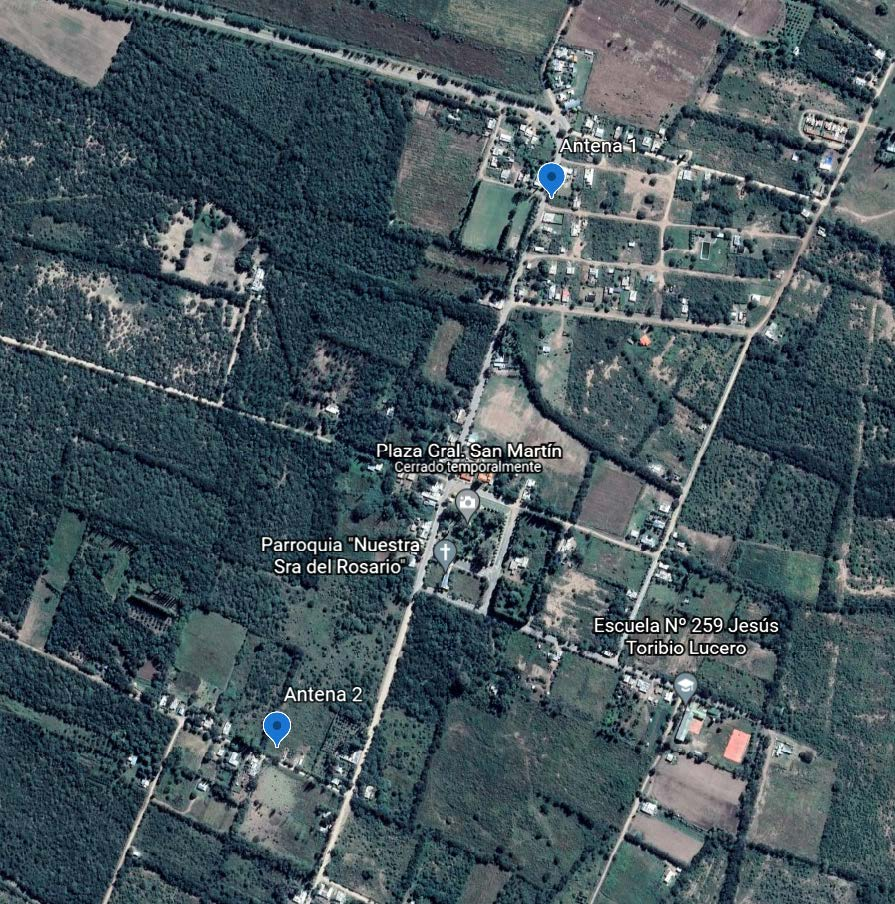
\includegraphics[width=0.7\linewidth]{fotos_ema/ubic_ap_alem.jpg}
  \caption{ubicación de los APs en la localidad de Leandro N. Alem.}
  \label{fig:ubic_ap_alem}
\end{figure}



Se decidió la ubicación de la antena 1 debido a la gran cantidad de edificaciones presentes, y si bien existe una antena de la competencia, esta presenta una gran cantidad de conectados, lo cual deviene en un peor servicio. 
Por otro lado, se decidió la ubicación de la antena 2, debido a que existe una cantidad importante de edificaciones, pero no se encuentran cubiertas por el rango de ninguna antena de la competencia. 
Teniendo esto en cuenta, cada equipo deberá lograr una tasa de transferencia bruta de por lo menos 985 Mbps.


\subsection{Armado de bases de datos para la simulación}
Para poder realizar la simulación, con la ayuda del programa AutoCAD se procede a realizar un trazado de los edificios y de la vegetación presente en la localidad. Luego trabajando con PropMan y Wallman se arma una base de datos para alimentar la simulación. Además es necesario realizar un modelado del patrón de radiación de la antena para ambas frecuencias y configurar las frecuencias con las que trabaja la antena, tanto para 2,4 GHz y 5 GHz. Esto es mostrado en mas detalle en el propio desarrollo del trabajo práctico de enlaces inalámbricos punto multi-punto \footnote{\href{https://docs.google.com/document/d/1Yf-dd03_VBnkoWaH1I282qp7TI3WjbeOEgkgxHz9xPk}{TRABAJO PRÁCTICO N$^{o}$ 3 "Enlaces Inalámbricos Punto Multi-Punto"}}.


Con los datos obtenidos en la simulación presente en el práctico, se realizó un análisis con el fin de obtener un radio aproximado de cobertura del servicio. 
Presentando nuevamente la tabla \ref{tab:area_24GHz} , se muestra una recopilación de los distintos radios mínimos medidos en el programa \textit{PropMan} para los distintos datos simulados. 
Teniendo en cuenta el datasheet del equipo elegido para la frecuencia de 2,4 GHz así como la modulación utilizada, se tiene una sensibilidad del receptor de -84 dBm. 
Con esto se procede a obtener un radio donde la potencia alrededor del equipo AP sea mayor que dicha sensibilidad. 
Por otro lado, se obtiene que según la modulación se necesita una SNR mínima de 18 dB. 
Sin embargo, por precaución, se toma un área circular donde la SNIR sea al menos mayor a 25 dB. 
Además, se obtiene el radio del área donde existe una probabilidad de conexión mayor al 80\%. 
Con estos datos se obtiene una posible área de cobertura del servicio. 
La posible área de cobertura se obtiene calculando un promedio de todos los valores, exceptuando la potencia mayor al umbral del receptor, al ser un valor muy alejado de la media. 
Con esto se obtiene un área de cobertura que abarca un radio de 487 metros para la primera antena, y de 483 metros para la segunda antena.

\begin{table}[htbp]
  \resizebox*{\textwidth}{!}{
    \begin{tabular}{|c|c|p{0.2\linewidth}|p{0.2\linewidth}|p{0.2\linewidth}|p{0.2\linewidth}|p{0.13\linewidth}|} \hline
\textbf{Frecuencia} & \textbf{Antena} & \textbf{Potencia mayor al umbral del receptor} & \textbf{Probabilidad de recepción mayor al 80\%} & \textbf{Alcance del data rate} & \textbf{SNIR mayor a 25 dB} & \textbf{Posible área de cobertura} \\ 
\hline 
\multirow{ 2}{*}{2,4 GHz} & Antena 1 & 900 & 500 & 710 & 250 & 487 \\ 
\cline{2-7}
 & Antena 2 & 1200 & 530 & 690 & 230 & 483 \\ 
 \hline 
\end{tabular}}
\caption{posible área de cobertura del servicio para 2.4 GHz.}
\label{tab:area_24GHz}
\end{table}


En el caso de la frecuencia de 5 GHz, se tiene un equipo con un umbral de recepción de -75 dBm para la modulación utilizada. 
Se procede a realizar lo mismo que se midió para la frecuencia de 2.4 GHz, sólo que en este caso se necesita un SNIR mayor a 24 dB. 
Para mayor seguridad se toma como mínimo un SNIR de 41 dB.  
Esto se muestra en la tabla \ref{tab:area_5GHz}.

\begin{table}[htbp]
  \resizebox*{\textwidth}{!}{
\begin{tabular}{|c|c|p{0.2\linewidth}|p{0.2\linewidth}|p{0.2\linewidth}|p{0.2\linewidth}|p{0.13\linewidth}|} \hline 
\textbf{Frecuencia} & \textbf{Antena} & \textbf{Potencia mayor al umbral del receptor} & \textbf{Probabilidad de recepción mayor al 80\%} & \textbf{Alcance del data rate} & \textbf{SNIR mayor a 41 dB} & \textbf{Promedio} \\ \hline 
\multirow{ 2}{*}{5 GHz} & Antena 1 & 300 & 310 & 415 & 200 & 308 \\ 
\cline{2-7} 
 & Antena 2 & 280 & 350 & 445 & 238 & 344 \\ \hline 
\end{tabular}}
\caption{Posible área de cobertura del servicio para 5 GHz.}
\label{tab:area_5GHz}
\end{table}

Finalmente, se esboza en AutoCAD la posible área de cobertura en donde se podría brindar el servicio. 
Esto se muestra en la Fig. \ref{fig:grafico_cobertura}, en donde con color rojo se marca el área cubierta por la antena 1, mientras que en azul el área cubierta por la antena 2.

\begin{figure}[ht!]
  \centering
  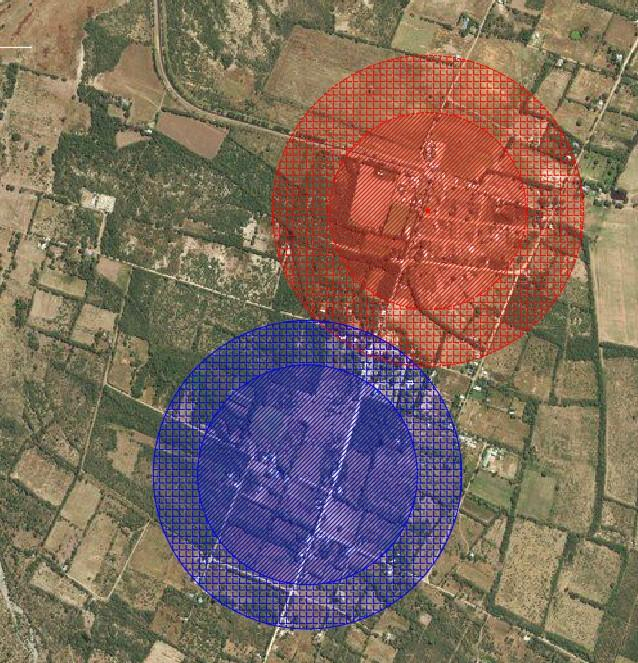
\includegraphics[width=0.8\linewidth]{fotos_ema/grafico_cobertura.jpg}
  \caption{Gráfico de la cobertura de ambas antenas.}
  \label{fig:grafico_cobertura}
\end{figure}

\subsection{Conslusión}

Con el análisis realizado, se puede concluir que el uso de 2 AP es suficiente para lograr la red propuesta y abarcar un total de 99 hogares, presentando así la cobertura suficiente para lograr los 83 clientes propuestos al inicio de este trabajo, ya que estos representan el 84\% del total abarcado. 

Por otro lado, con la configuración elegida no se logró la tasa de transferencia bruta propuesta al inicio de este trabajo de 985 Mbps para cada AP. No obstante, esto no supondrá un problema ya que debido al sobredimensionamiento que se utilizó para el cálculo, se optó por una configuración que brinde una tasa de transferencia bruta de 967 Mbps, pero que abarque la mayor área posible.



\section{Red de acceso con fibra óptica}

\subsection{Determinación de la cantidad de ONTs que soporta cada OLT}

Del estudio socioeconómico realizado sobre la localidad de Leandro N. Alem se obtuvo que 83 hogares del total de la población serán potenciales clientes del servicio brindado. 
Además, se obtuvo que la tasa de transferencia requerida por cliente teniendo en cuenta el peor de los casos es de 11,86 Mbps.

Para calcular el número máximo de ONTs que soporta una OLT por puerto se utiliza la ecuación \ref{eq:max_ont}.

\begin{equation}
 C*B*TCP=CRG
 \label{eq:max_ont}
\end{equation}


Donde:

\begin{itemize}
\item  $C$ = Tasa de concurrencia
\item  $N$ = Número de ONT
\item  $TCP$ = Tráfico por cliente
\item  $CRG$ = Capacidad de la red GPON
\end{itemize}

Sabiendo que la capacidad de la red GPON es de 1,25 Gbps, el número y el tráfico por clientes es el mencionado anteriormente y considerando una tasa de concurrencia del 100\%, reemplazando en la ecuación \ref{eq:max_ont} se obtiene que cada puerto de la OLT puede manejar un máximo de 101 ONTs como muestra la ecuación \ref{eq:res_ont_max}.

\begin{equation}
  N=\frac{CRG}{C*TCP}=\frac{1200*10^6}{1*11,86*10^6}\approx 101  
  \label{eq:res_ont_max}
\end{equation}

Como conclusión se obtiene que al tener una tasa de concurrencia del 100\%, con un puerto GPON de la OLT es suficiente para manejar los 83 clientes de la localidad de Leandro N. Alem.


%================================================================

\subsection{Determinación del alcance de la red óptica}

\subsubsection{OLT}

Para determinar el alcance de la red óptica es menester elegir los distintos equipos que la conforman. 
Primeramente, se preseleccionaron los siguientes OLTs de las marcas Ubiquiti y TP-Link, debido a que son marcas comercializadas ampliamente en Argentina y disponen de revendedores en el país. 
Las características de los mismos son mostradas en la tabla \ref{tab:olts_presel}.

\begin{table}[htbp]
  \centering
  \begin{tabular}{|c|c|c|c|} \hline 
    \textbf{Opciones} & \textbf{Opción 1} & \textbf{Opción 2} & \textbf{Opción 3} \\ \hline 
    \textbf{Marca} & Ubiquiti & Ubiquiti & TP-Link \\ \hline 
    \textbf{Modelo} & UF-OLT\tablefootnote{\href{https://dl.ubnt.com/ds/uf_gpon}{UFiber GPON Datasheet, página 9}} & UF-OLT-4\tablefootnote{\href{https://dl.ubnt.com/ds/uf_gpon}{UFiber GPON Datasheet, página 10}} & OLT P1201-08\tablefootnote{\href{https://www.tp-link.com/ar/service-provider/gpon/p1201-08/}{P1201-08|GPON OLT de 8 puertos}} \\ \hline 
    \textbf{Puertos GPON SFP} & 8 & 4 & 8 \\ \hline 
    \textbf{Puertos SFP+} & 2 & 1 & 2 \\ \hline 
    \textbf{Cantidad de ONUs máxima} & 1024 & 512 & 1024 \\ \hline 
    \textbf{Precio con un dólar a \$ 165} & \$ 1.385,27 & \$ 890,53 & \$ 1.447,85 \\ \hline 
    \textbf{Precio en pesos} &  \$ 228.569,00\tablefootnote{\href{https://articulo.mercadolibre.com.ar/MLA-730499098-ufiber-ubiquiti-uf-olt-8-puertos-gpon-sfp-linea-optica-_JM}{Precio opción 1}} &  \$ 146.937,00\tablefootnote{\href{https://www.mercadolibre.com.ar/switch-ubiquiti-networks-uf-olt-4/p/MLA14615949}{Precio opción 2}} &  \$ 238.896,00\tablefootnote{\href{https://articulo.mercadolibre.com.ar/MLA-926970453-switch-router-tp-link-p1201-08-8-puertos-gpon-olt-4-giga-sfp-_JM}{Precio opción 3}} \\ \hline 
    \end{tabular}
    \caption{opciones de OLTs preseleccionados.}
    \label{tab:olts_presel}  
\end{table}

Analizando las opciones encontradas, se tiene que la opción 2 posee la menor cantidad de puertos SFP y SFP+ de todos los equipos. 
No obstante, considerando que la cantidad de clientes máximos soportada por cada equipo excede en gran manera a la cantidad de clientes previstos, la cantidad de puertos no es un elemento decisivo. 

Por otro lado, las opciones 1 y 2 incluyen un módulo SFP clase B+\footnote{\href{https://docs.google.com/spreadsheets/d/1rmlMl8y5O11057Wbb303iKk9dc6XedijkpFMKAgwH_U/edit\#gid=2076166277}{Lista de Precios - LQ.xlsx, Libro: Ubiquiti, Celda: B157}}, modelo UF-GP-B+\footnote{\href{https://www.ui.com/accessories/gpon-network-accessories/}{GPON Network Accessories}}.
Según lo calculado en el apartado anterior, con un solo puerto GPON se puede cubrir los requerimientos de la red deseada. 
Es por ello, que el hecho de contar con un módulo SFP GPON incluido presenta una gran ventaja, ya que se evita la necesidad de buscar un dispositivo y se obtiene un equipo listo para ser instalado, con una compatibilidad asegurada por el fabricante. 
Este ahorro de dinero en la inversión inicial es fundamental para poder asegurar un servicio lo más económico posible. 
Es por ello, que se descarta la opción 3. 

Finalmente se elige la opción 2, ya que es la más económica, presenta la cantidad de puertos suficiente para la implementación de la red y además se comercializa con un módulo SFP incluido en el costo. 
Si al realizar el cálculo de enlace no se cumple con el presupuesto de potencia, se comercializan también módulos SFP clase C+ de la misma marca. 

\subsubsection{Módulos SFP}
Se presenta en la tabla \ref{tab:comp_sfp} una comparativa entre el módulo SFP clase B+ y clase C+.
\begin{table}[htbp]
  \centering
\begin{tabular}{|c|c|c|} \hline 
\textbf{Opciones} & \textbf{Opción 1} & \textbf{Opción 2} \\ \hline 
\textbf{Marca} & Ubiquiti & Ubiquiti \\ \hline 
\textbf{Modelo} & UF‑GP‑B+\footnote{\href{}{UFiber GPON Datasheet, página 5}} & UF‑GP‑C+ \\ \hline 
\textbf{Precio en dólares} & \$ 166,36 & \$117\footnote{\href{}{Lista de Precios - LQ.xlsx, celda A159}} \\ \hline 
\textbf{Precio en pesos} & \$ 27.450,00\footnote{\href{}{Precio opción 1}} & \$ 14.263,00 \\ \hline 
\textbf{Módulo Óptico} & Clase B+ & Clase C+ \\ \hline 
\textbf{Rango de potencia TX} & 1,5 a 5 dBm & 3 a 7 dBm \\ \hline 
\textbf{Rango de potencia RX} & -28 a -8 dBm & -32 a -12 dBm \\ \hline 
\textbf{Longitud de onda TX} & 1490 nm & 1490 nm \\ \hline 
\textbf{Longitud de onda RX} & 1310 nm & 1310 nm \\ \hline 
\end{tabular}
\caption{Comparativa entre los 2 modulos SFP.}
\label{tab:comp_sfp}
\end{table}


\subsubsection{ONT/ONU}

En el caso de las ONUs, se presentan en la tabla \ref{tab:comp_onus} tres opciones con sus respectivas características. Debido a que el módulo SFP que incluye el equipo previamente elegido es de clase B+, se descarta la opción 3, ya que es de clase C+. Se opta por elegir la opción 2, debido a que es la más económica y presenta las mismas características que la opción 1.
\begin{table}[htbp]
  \centering
\begin{tabular}{|c|c|c|c|} \hline 
\textbf{Opciones} & \textbf{Opción 1} & \textbf{Opción 2} & \textbf{Opción 3} \\ \hline 
\textbf{Marca} & Ubiquiti & TP-Link & TP-Link \\ \hline 
\textbf{Modelo} & UF-Loco\tablefootnote{\href{https://dl.ubnt.com/ds/uf_gpon}{UFiber GPON Datasheet, página 12}} & XZ000-G3\tablefootnote{\href{https://www.tp-link.com/ar/service-provider/gpon/xz000-g3/\#specifications}{XZ000-G3 | Terminal GPON Gigabit de 1 puerto}} & TX-6610\tablefootnote{\href{https://www.tp-link.com/ae/service-provider/gpon/tx-6610/\#specifications}{TX-6610 |1-Port Gigabit GPON Terminal}} \\ \hline 
\textbf{Precio en dólares} &  \$ 54,0 &  \$ 14,8 &  \$ 20 \\ \hline 
\textbf{Precio en pesos} &  \$ 5.997,0\tablefootnote{\href{https://docs.google.com/spreadsheets/d/1rmlMl8y5O11057Wbb303iKk9dc6XedijkpFMKAgwH_U/edit\#gid=2076166277}{Precio opción 1}} &  \$ 2.450,0\tablefootnote{\href{https://articulo.mercadolibre.com.ar/MLA-926563889-terminal-gpon-gigabit-de-1-puerto-tp-link-xz000-g3-_JM}{Precio opción 2}} &  \$ 3.300,0\tablefootnote{\href{https://articulo.mercadolibre.com.ar/MLA-856287978-modem-terminal-gpon-tp-link-fibra-optica-giga-voip-ftth-_JM}{Precio opción 3}} \\ \hline 
\textbf{Módulo Óptico} & Clase B+ & Clase B+ & Clase C+ \\ \hline 
\textbf{Rango de potencia TX} & 1,5 a 5 dBm & 1,5 a 5 dBm & 3 a 7 dBm \\ \hline 
\textbf{Rango de potencia RX} & -28 a -8 dBm & -28 a -8 dBm & -32 a -12 dBm \\ \hline 
\end{tabular}
\caption{ONUs preseleccionadas.}
\label{tab:comp_onus}
\end{table}

\subsubsection{Fibra óptica:}

Para la distribución de la fibra óptica se deciden utilizar 2 tipos teniendo en cuenta cuál se adapta mejor a cada escenario. 
Desde el OLT hasta el splitter se utilizará el tipo de fibra óptica G.652.D. 
Esto se debe a que se comercializa en bobinas de 4 km, lo cual permitiría reducir los empalmes necesarios para llegar al splitter. 
Por otro lado, del splitter hasta el equipo ONT/ONU se decide utilizar la fibra óptica G.657.A porque tiene menores pérdidas ante los dobleces, permitiendo resistir mejor una instalación domiciliaria. 
Para ello se consideran las siguientes opciones de cables:

\begin{itemize}
\item  Cable ADSS, de la marca GLC, modelo GLC-ADSS80-4/6 y se comercializa en bobinas de 4 km\footnote{\href{https://docs.google.com/spreadsheets/d/1rmlMl8y5O11057Wbb303iKk9dc6XedijkpFMKAgwH_U/edit\#gid=400833791}{Lista de Precios - LQ.xlsx, Libro: Fibra-GLC, Celda A14, CATÁLOGO, página 27}}. La fibra corresponde a la norma G.652.D.
\item  Cable Drop FTTH FLAT con portante de dieléctrico, modelo GLC-DROP-FLAT-DIE, se comercializa en bobinas de 2 km y la fibra óptica se corresponde con G.657.A1\footnote{\href{https://docs.google.com/spreadsheets/d/1rmlMl8y5O11057Wbb303iKk9dc6XedijkpFMKAgwH_U/edit\#gid=400833791}{Lista de Precios - LQ.xlsx, Libro: Fibra-GLC, Celda A38, CATÁLOGO, página 30}}. Además presenta la opción de 1, 2 o 4 pelos de fibra óptica.
\item  Cable Drop Profiber de 1 pelo de fibra óptica, es del tipo G.657.A2 LSZH (SM) ANTI FLAMA con mensajero de ACERO y se comercializa en bobinas de 1 km\footnote{\href{https://docs.google.com/spreadsheets/d/1rmlMl8y5O11057Wbb303iKk9dc6XedijkpFMKAgwH_U/edit\#gid=400833791}{Lista de Precios - LQ.xlsx, Libro: Fibra Profiber, Celda A27,FIBRA OPTICA DROP}}. 
\end{itemize}

Teniendo en cuenta que las fibras ópticas del tipo G.657 de la categoría A son totalmente compatibles con las fibras monomodo UIT-T G.652, se decide utilizar la fibra óptica tipo G.657.A2 ya que esta posee mayor resistencia a los dobleces que la fibra del tipo G.657.A1. 
Para la transmisión, los equipos utilizan las longitudes de onda 1490 nm y 1310 nm. 
Esto deviene en que para el cálculo de enlace, las atenuaciones de las fibras según las hojas de datos son: 

\begin{itemize}
\item  Para 1310: 0,35 dB/km
\item  Para 1490: 0,25 dB/km 
\end{itemize}

En la sección \ref{section:calculo_alc_max_fo} del anexo, se obtuvo que las distancias máximas para el upstream es de 85,67 kilómetros y de 116,8 kilómetros para el downstream.
Es menester recalcar que si bien la distancia máxima que se puede lograr en teoría es mayor a los 20 kilómetros que el equipo marca como máximo, al utilizar un splitter, las pérdidas que este presenta pueden variar desde los 5 hasta los 25 decibelios, disminuyendo la distancia efectiva del enlace. 
Esto será abordado con más detalle en el siguiente apartado.
  
%=================================================================
\subsection{Splitters}
  
En la sección \ref{section:calc_rel_div_spl} del anexo se presentan las características de las distintas opciones de splitters considerados para el proyecto.    
Si bien los splitters de la marca MACH tienen menor atenuación, se elige trabajar con los productos de la marca KOC debido a que se obtuvo información de los precios por parte del fabricante a través de un presupuesto enviado por e-mail. 

\subsection{Representación esquemática de la solución de OLTs, splitters y ONTs}
    
Del estudio realizado en la sección  sobre la distribución de los potenciales clientes se obtuvo que el 80 \% (66 clientes) de la población vive en los cuadrantes del 1 al 9 y el 20\% restante (17 clientes) se encuentra distribuido entre los cuadrantes 10 al 15.
En la Fig. \ref{fig:cuadrantes_alem_fo} se observa en rojo los cuadrantes en los cuales se concentra la mayor cantidad de gente y con un icono verde la ubicación de las antenas de la Autopista de la Información. 
Con las imágenes aéreas provistas por el software Google Earth y con la imposibilidad de realizar un sondeo económico de la zona, se estimó que los clientes con mayor poder adquisitivo se encuentran entre los cuadrantes que van del 1 al 6, dado el mayor tamaño de la vivienda respecto a las demás. 
Sin embargo se decidió dar prioridad a los cuadrantes 3, 4, 5 y 6 dada la ubicación de una antena de internet de la competencia. 
Por otra parte, los cuadrantes del 11 al 14 no se ven alcanzados por ninguna antena del gobierno, por lo que se estima que brindando un servicio que antes no disponían se encontrarán potenciales clientes en esta zona. 
Por último, en los cuadrantes 9 y 10 está la zona céntrica, en la cual se ubica la plaza donde se encuentra una antena de internet de la competencia que está saturada. 


\begin{figure}[htbp]
  \centering
  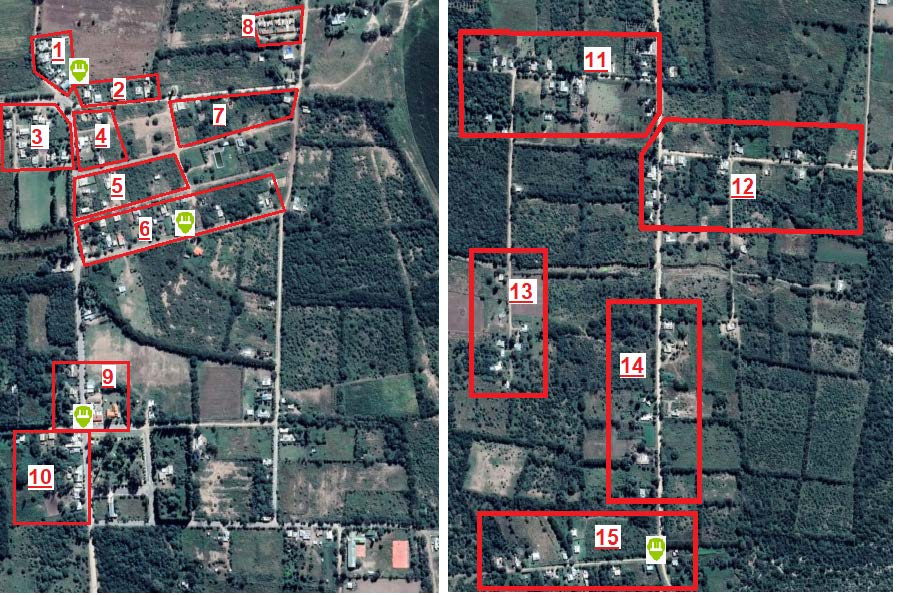
\includegraphics[width=0.8\linewidth]{fotos_ema/cuadrantes_alem.jpg}
  \caption{a la izquierda la zona norte y a la derecha la zona sur de la localidad de leandro N. Alem.}
  \label{fig:cuadrantes_alem_fo}
\end{figure}



\part{Comparación de ambas soluciones}



\begin{table}[htbp]
  \resizebox{\textwidth}{!}{
  \centering
    \begin{tabular}{|c|C{0.25\textwidth}|C{0.25\textwidth}|C{0.25\textwidth}|C{0.25\textwidth}|}
\cline{2-5}    \multicolumn{1}{r|}{} & \multicolumn{2}{c|}{Radio Enlace} & \multicolumn{2}{c|}{Fibra óptica} \bigstrut\\
\cline{2-5}    \multicolumn{1}{r|}{} & Ventajas & Desventajas & Ventajas & Desventajas \bigstrut\\
\hline
    \multirow{6}[12]{*}{Troncal} & Equipamiento e instalaciones económicas & La torre resulta intrusiva al paisaje natural & No se necesita infraestructura nueva para el tendido. & Altos costos \bigstrut\\
\cline{2-5}         & Fácil adquisición de materiales y equipos & Permisos  de construcción y edificación & Facilidad para extender el servicio a otras localidades & Gran cantidad de equipos necesarios para el tendido \bigstrut\\
\cline{2-5}         & Existe posibilidad de proveer una mayor tasa de transferencia sin necesidad de cambiar el equipo & Si se desea ampliar el servicio a otras zonas, se debe comprar nuevos equipos y colocar nuevas torres & Baja latencia & Se requieren cuidados especiales en el despliegue \bigstrut\\
\cline{2-5}         & No necesita de un mantenimiento regular & El servicio es afectado por las inclemencias del tiempo & Alta fidelidad, independiente de las inclemencias del tiempo & Alto mantenimiento, debido a posibles cortes en la fibra \bigstrut\\
\cline{2-5}         & Instalación y puesta en marcha & Necesita de técnicos capacitados en trabajo en altura para su mantenimiento & Posibilidad de partnership con el gobierno de San Luis & Instalación y puesta en marcha \bigstrut\\
\cline{2-5}         & Debido a la frecuencia utilizada, no es necesario licencias ni pago de comisiones &  &      & Lenta amortización \bigstrut\\
\hline
    \multirow{6}[12]{*}{Distribución} & Facilidad de conexión para nuevos usuarios & El servicio es afectado por las inclemencias del tiempo & Robustez ante ataques informáticos & Altos costos de mantenimiento y despliegue \bigstrut\\
\cline{2-5}         & Baja cantidad de equipos necesarios para brindar el servicio & Posibilidad de phishing & Brindar un servicio no existente, alternativo al competidor principal & Baja flexibilidad a la hora de incorporar nuevos clientes \bigstrut\\
\cline{2-5}         & Bajo requerimiento de fibra óptica & Complicaciones a la hora de aumentar la cobertura & Altas tasas de transferencia &  \bigstrut\\
\cline{2-5}         & Bajo mantenimiento & Reducción del ancho de banda en horas pico & Baja latencia &  \bigstrut\\
\cline{2-5}         &      & Posibilidad de hurto de los equipos & Baja probabilidad de hurto de los equipos &  \bigstrut\\
\cline{2-5}         &      & Problemas a la hora de establecer el enlace  con las obstrucciones  &      &  \bigstrut\\
    \hline
    \end{tabular}}%
    \caption{Comparación de ambas tecnologías tanto para red de acceso como red de distribución.}
  \label{tab:comp_tec}%
\end{table}%



\part{Análisis económico}

La realización de un análisis económico y financiero es fundamental para poder evaluar distintos aspectos vinculados con el proyecto y su evolución. 

El análisis económico y financiero del proyecto apunta a:

\begin{itemize}
    \item Conocer en detalle los costos individuales y totales involucrados, tanto en el proceso de desarrollo como en la implementación y gestión del proyecto a lo largo del tiempo.
    \item Identificar las necesidades de fondeo externo o propio a lo largo de la vida del proyecto. 
    \item Proyectar las ventas potenciales y registrar las ventas reales que tenga el proyecto en sus distintas etapas. 
    \item Identificar las variables externas e internas que impactan en el proyecto y analizar cómo estas variables pueden sensibilizar la evolución y los resultados parciales y totales del mismo. 
    \item Conocer los impactos económicos directos e indirectos del proyecto en forma cuantitativa.
\end{itemize}

En conjunto, el análisis económico y financiero permite conocer la viabilidad concreta del proyecto a lo largo de las distintas etapas y su sustentabilidad real en el mediano y largo plazo. 

\section{Costo de capital (CAPEX)}

 En esta categoría se engloba todas aquellas compras e inversiones en activos físicos que aumentan la capacidad productiva de la empresa y que pasan a formar parte de su propiedad.

***Al mismo tiempo, también incluye los gastos de mantenimiento destinados a expandir la vida útil de los equipos utilizados. ***

\subsection{Red de transporte cableado}

Realizando una investigación de mercado se cotizaron los equipos activos y materiales elegidos en la Parte IV. Los mismos se muestran en la tabla

\begin{table}[htbp]
  \centering
  \resizebox*{\textwidth}{!}{
    \begin{tabular}{ccccc|c|c|}
    \hline
    \multicolumn{1}{|c|}{Red Troncal} & \multicolumn{1}{c|}{Descripción} & \multicolumn{1}{c|}{Modelo} & \multicolumn{1}{c|}{Marca} & Cantidad  & Costo unitario  & Costo total (US\$) \bigstrut\\
    \hline
    \multicolumn{1}{|c|}{\multirow{3}[6]{*}{Insumos}} & \multicolumn{1}{p{10.43em}|}{Fibra óptica monomodo 4km/rollo} & \multicolumn{1}{c|}{GLCADSS80-12} & \multicolumn{1}{c|}{GLC} & 16    & 1745  & 27.920 \bigstrut\\
\cline{2-7}    \multicolumn{1}{|c|}{} & \multicolumn{1}{p{10.43em}|}{Gabinete para exterior Botella de empalme 12/48} & \multicolumn{1}{c|}{F01S200} & \multicolumn{1}{c|}{Fujie} & 16    & 30,3    & 484,8 \bigstrut\\
\cline{2-7}    \multicolumn{1}{|c|}{} & \multicolumn{1}{p{10.43em}|}{Conectores Pigtail Patchcord} & \multicolumn{1}{c|}{FO-2537} & \multicolumn{1}{c|}{GLC} & 2     & 3,21   & 6,42 \bigstrut\\
    \hline
    \multicolumn{1}{|c|}{\multirow{3}[6]{*}{Equipos activos}} & \multicolumn{1}{p{10.43em}|}{Tranceptores Transmisores/Reseptores} & \multicolumn{1}{c|}{SFP-GE-BX80} & \multicolumn{1}{c|}{FS} & 2     & 52    & 104,00 \bigstrut\\
\cline{2-7}    \multicolumn{1}{|c|}{} & \multicolumn{1}{p{10.43em}|}{Switch 48 puertos RJ-45, 2 puertos SFP, 2 puertos SFP+} & \multicolumn{1}{c|}{ES-48-LITE} & \multicolumn{1}{p{4.715em}|}{Ubiquiti Networks} & 2     & 752   & 1.504,00 \bigstrut\\
\cline{2-7}    \multicolumn{1}{|c|}{} & \multicolumn{1}{p{10.43em}|}{UPS Rango de voltaje de entrada es de 176V - 294V} & \multicolumn{1}{c|}{BR900G} & \multicolumn{1}{c|}{APC} & 2     & 250   & 500,00 \bigstrut\\
    \hline
    \multicolumn{5}{c|}{}                 & TOTAL: & 30.519 \bigstrut\\
\cline{6-7}    
\end{tabular}}%
\caption{Add caption}
  \label{tab:addlabel}%
\end{table}%



\subsection{Red de distribución GPON}.

De la misma forma que en el punto anterior, se elige luego de varias cotizaciones, los materiales para la red de distribución mostrados en la tabla 

\subsection{Costo de instalación}.



\section{Costo operativos (OPEX)}

En esta sección se consideran los gastos relacionados con la administración de la red y mantenimiento. Los gastos requeridos para el personal técnico, publicidad y alquileres también son tenidos en cuenta. 

\subsection{Costo de servicios}.

Son aquellos gastos requeridos para mantener la red operativa.

\subsubsection{Consumo Electrico}

El consumo eléctrico es la cantidad de energía demandada por un determinado punto de suministro durante un plazo de tiempo denominado período de facturación. Este es facturado en la provincia de San Luis por EDESAL S.A. Utilizando el cuadro tarifario disponible en su pagina web\footnote{\href{https://oficinavirtualedesal.com.ar/ove/html/simulacion.html}{EDESAL}} se puede calcular el costo de energía eléctrica utilizado por la red.
En la tabla se puede observar el consumo correspondiente en la sea cada componente activo del sistema.

Considerando que los equipos estan activos todo el tiempo, segun el cuadro tarifario, el gasto mensual corresponde a 

\subsubsection{Internet}

Debido al congelamiento de precios realizados por el gobierno nacional, el precio del megabit mayorista era al 31 de enero de 2020 de 447 pesos argentinos
\footnote{\href{https://www.argentina.gob.ar/noticias/el-gobierno-congela-el-precio-de-internet-mayorista-de-arsat\#:~:text=El\%20vicejefe\%20de\%20Gabinete\%20y,de\%20$447\%20pesos\%20por\%20mega.}{El Gobierno congela el precio de internet mayorista de ARSAT}}.
Teniendo en cuenta que el precio del megabit se actualiza a partir del índice de precios al consumidor, el precio al mes de junio de 2021 correspondería a 738 pesos argentinos\footnote{\href{https://calculadoradeinflacion.com/argentina.html?md=enero&ad=2020&mh=junio&ah=2021&q=447}{Calculadora de inflación
histórica de Argentina}}, o US\$4,47 dólares con un dolar a 165 pesos argentinos.

Con este precio se obtiene el monto total en dólares del servicio contratado a ARSAT. 
Esto se muestra en la ecuación \ref{eq:costo_may_internet}.

\begin{eqnarray}
    \text{Costo de internet }&=&\text{Megabits necesarios}*\text{Precio del megabit mayorista}\\
    &=&255\text{ Megabits}*\text{US}\$4,47\approx\text{US}\$1140 \nonumber
    \label{eq:costo_may_internet}
\end{eqnarray}

\subsubsection{IPTV}

El gasto correspondiente al servicio de IPTV se estima a partir del costo minorista de un servicio con características similares a las brindadas en este proyecto. De esta forma, el servicio minorista tiene un valor alrededor de los US\$ 15 \footnote{\href{https://compraonline.telecom.com.ar/producto/telecomunicaciones/tv-por-cable}{Telecom}}. Estimando que el costo mayorista es un 30\% del costo minorista:

\begin{equation}
    \text{Costo mayorista servicio IPTV p/ abonado } = \text{US}\$ 15 * 0,3 = \text{US}\$ 4,5 
\end{equation}

\subsubsection{VoIP}

Debido a su utilidad en decremento en la actualidad,se considera que la cantidad de clientes que utilizaran el servicio de VoIP es menor al 15\%.
Considerando que el tráfico por móvil se encuentra alrededor de los 25 mE y la cantidad de clientes que utilizan el servicio es de 13 clientes, se obtiene que el trafico en la hora pico esta dado por la ecuación \ref{eq:bht}

\begin{equation}
    BHT = \text{Tráfico por móvil} * \text{Clientes} = 0,025 * 13 = 0,325 \text{ Erlang}
    \label{eq:bht}
\end{equation}

Para calcular cantidad de canales de voz se consideró que la probabilidad de bloqueo de
llamadas era del 2\% y en base al resultado obtenido en la Ecuación \ref{eq:bht} se utilizó la calculadora online Erlang B2\footnote{\href{https://www.erlang.com/calculator/erlb/}{Erlang}}. 
La calculadora Erlang B calcula la cantidad de líneas de voz (n úmero de circuitos en un grupo troncal) necesarias a partir de 2 variables:
\begin{itemize}
    \item Tráfico de horas ocupadas (en Erlangs): las horas de tráfico de llamadas durante la hora de mayor actividad de funcionamiento de un sistema telefónico.
\item Bloqueo: la proporción de llamadas que fallan por líneas insuficientes.
\end{itemize}

En la figura \ref{fig:erla} se observa como resultado que el curso total de trafico es equivalente a tener 3 canal de voz permanentemente activa. 

\begin{figure}[htbp]
  \centering
  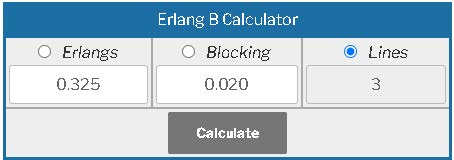
\includegraphics[width=0.6\linewidth]{fotos_julian/erlang}
  \caption{Calculo del trafico total.}
  \label{fig:erla}
\end{figure}

La cotización brindada por la empresa Dainus\footnote{\href{https://dainus.net/sip}{Dainus}} corresponde a US\$ 7,27 mensuales para el pack SIP Trunk 1, ofreciendo hasta 5 llamadas simultaneas, lo cual cubre los requisitos planteados.   



\part{Propuesta de la empresa}

Considerando lo analizado en la tabla \ref{tab:comp_tec} de la parte V y el análisis económico previamente explicado se opta por realizar una instalación de fibra óptica tanto para la red troncal como para red de acceso.
En la elección se tuvo en cuenta el siguiente análisis: 


\part{Conclusiones}

\part{Anexos y referencias}

\section{Cálculo del alcance máximo de la red óptica}
\label{section:calculo_alc_max_fo}
Una vez elegidos los equipos con sus respectivas características, para el cálculo del alcance máximo de la red óptica se utiliza la siguiente ecuación \ref{eq:alc_max_ro}. 
\begin{equation}
  P \geq D*P_{fo}+E*P_e+C*P_c+S+F
  \label{eq:alc_max_ro} 
\end{equation}

donde,

\begin{itemize}
\item  $P$ representa el saldo de potencia OLT-ONU. Como se desea obtener la máxima distancia posible, se considera $P=P_{TXmaxima}-S_{RXminima}=5-(-28)=33$dBm
\item  $D$ representa la distancia máxima OLT-ONU, en kilómetros.
\item  $P_{fo}$ representa la pérdida en la fibra óptica en dB/km.
\item  $E$ representa la cantidad de empalmes.
\item  $P_e$ representa las pérdidas por empalme en dB.
\item  $C$ representa la cantidad de conectores.
\item  $P_c$ representa las pérdidas por conector en dB.
\item  $S$ representa las pérdidas por splitter en dB.
\item  $F$ representa el factor de proyecto que prevé futuras pérdidas o degradaciones de la fibra óptica.
\end{itemize}

Previo al cálculo de la distancia, es necesario analizar más en detalle cómo se distribuirá la fibra óptica a lo largo de nuestra red. 
Para ello, se plantea la posibilidad de usar la mayor cantidad de bobinas de 4 km, llevando el splitter lo más cerca del usuario final y usar solamente una bobina de la fibra óptica DROP para llegar desde el splitter hasta la ONU. 
Esto se decide para evitar empalmes. 
El conexionado presentará en total 4 conectores, 2 en el tramo OLT-Splitter y 2 en el tramo Splitter-ONU. 
En la Fig. \ref{fig:esq_dist_max} se muestra un pequeño esquema de la conexión, el cual permitirá calcular la distancia máxima posible entre la OLT y la ONU.

\begin{figure}[htbp]
  \centering
  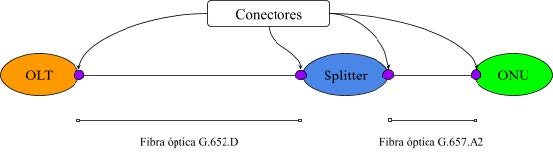
\includegraphics[width=0.8\linewidth]{fotos_ema/esq_dist_max.jpg}
  \caption{Esquema de conexiones planteado para obtener la distancia máxima.}
  \label{fig:esq_dist_max}
\end{figure}

%=========================================================================================


Reescribiendo la cantidad de empalmes, ya que estos dependen de la distancia y debido a que no se tienen en cuenta las pérdidas por splitters y el margen de seguridad, la distancia teórica se obtiene con el siguiente planteo:
\begin{equation}
  P \geq {(D}_{G652D}+D_{G657A2})*P_{fo}+\left(\frac{D_{G652D}}{L_{B_{G652D}}}+\frac{D_{G657A2}}{L_{B_{G657A2}}}\right)*P_e+C*P_c
\end{equation}
 
donde

\begin{itemize}
  \item  $D_{G652D}$ es la distancia que se recorre con la fibra tipo G.652.D.
  \item  $D_{G657A2}$ es la distancia que se recorre con la fibra tipo G.657.A2.
  \item  $L_{B_{G652D}}$ es la longitud de la bobina de la fibra tipo G.652.D.
  \item  $L_{B_{G657A2}}$ es la longitud de la bobina de la fibra tipo G.657.A2.
  \end{itemize}
  
  Considerando lo planteado previamente:

  \begin{eqnarray*}
    P &\geq& {(D}_{G652D}+1)*P_{fo}+\left(\frac{D_{G652D}}{4}+1\right)*P_e+4P_c \\
    P &\geq& D_{G652D}P_{fo}+P_{fo}+\frac{D_{G652D}}{4}P_e+P_e+4P_c \\
    P-P_{fo}-P_e-4P_c &\geq& D_{G652D}\left(P_{fo}+\frac{P_e}{4}\right)  \\
    \frac{P-P_{fo}-P_e-4P_c}{\left(P_{fo}+\frac{P_e}{4}\right)} &\geq& D_{G652D}
  \end{eqnarray*}
  
  Considerando conectores con pérdidas de 0,2 dB y pérdidas por empalmes de 0,1 dB, se procede a obtener la distancia máxima para el upstream. Con una longitud de onda de 1310 nm, se obtiene que la distancia máxima es:

  \begin{eqnarray*}
    \frac{33-0.35-0.1-4*0.2}{\left(0.35+\frac{0.1}{4}\right)} &\geq& D_{G652D} \\
    84.67 &\geq& D_{G652D} \\
    D&=&D_{G652D}+D_{G657A2}=85.67 \text{ kilómetros}
  \end{eqnarray*}

  
  Para el downstream, operando con una longitud de onda de 1490 nm, se obtiene que la distancia máxima es:
  \begin{eqnarray*}
    \frac{33-0.25-0.1-4*0.2}{\left(0.25+\frac{0.1}{4}\right)}&\geq& D_{G652D} \\
    115.8 &\geq& D_{G652D} \\
    D&=&D_{G652D}+D_{G657A2}=116.8 \text{ kilómetros}
  \end{eqnarray*}


  \section{Cálculo de la relación de división de los splitters a instalar tras cada OLT}
  \label{section:calc_rel_div_spl}

  Teniendo en cuenta la disponibilidad de splitters que se comercializan, se obtienen splitters con una relación desde 1:2 a 1:128\footnote{\href{https://www.koc.com.ar/productos-redes-de-fibra-optica/splitter-plc-plc-1xn/}{Splitter PLC conectorizado -- KOC Latinoamérica}}. 
  Para obtener los 101 ONTs calculados, se procede a plantear las posibles combinaciones necesarias para cubrir dicha cantidad. 
  Teniendo en cuenta que por cada etapa de multiplexación el enlace sufre de mayores pérdidas, además de complejizarse el mantenimiento y la distribución de la red, la multiplexación propuesta presentará 2 etapas. 
  Para el enlace, se consideraron 2 marcas comercializadas en Argentina, KOC y MACH. 
  
  Las características de los splitters KOC no están disponibles al público, por lo cual fueron solicitados por mail, al igual que su precio. 
  En el caso de la marca MACH se obtuvieron las características pero no información del precio. 
  A continuación, se muestran las capturas de las hojas de datos provistas por los fabricantes previamente mencionados. 



  \begin{itemize}
    \item  MACH electronics, presenta las características mostradas en la Fig. \ref{fig:splitters_mach}.

    \begin{figure}[htbp]
      \centering
      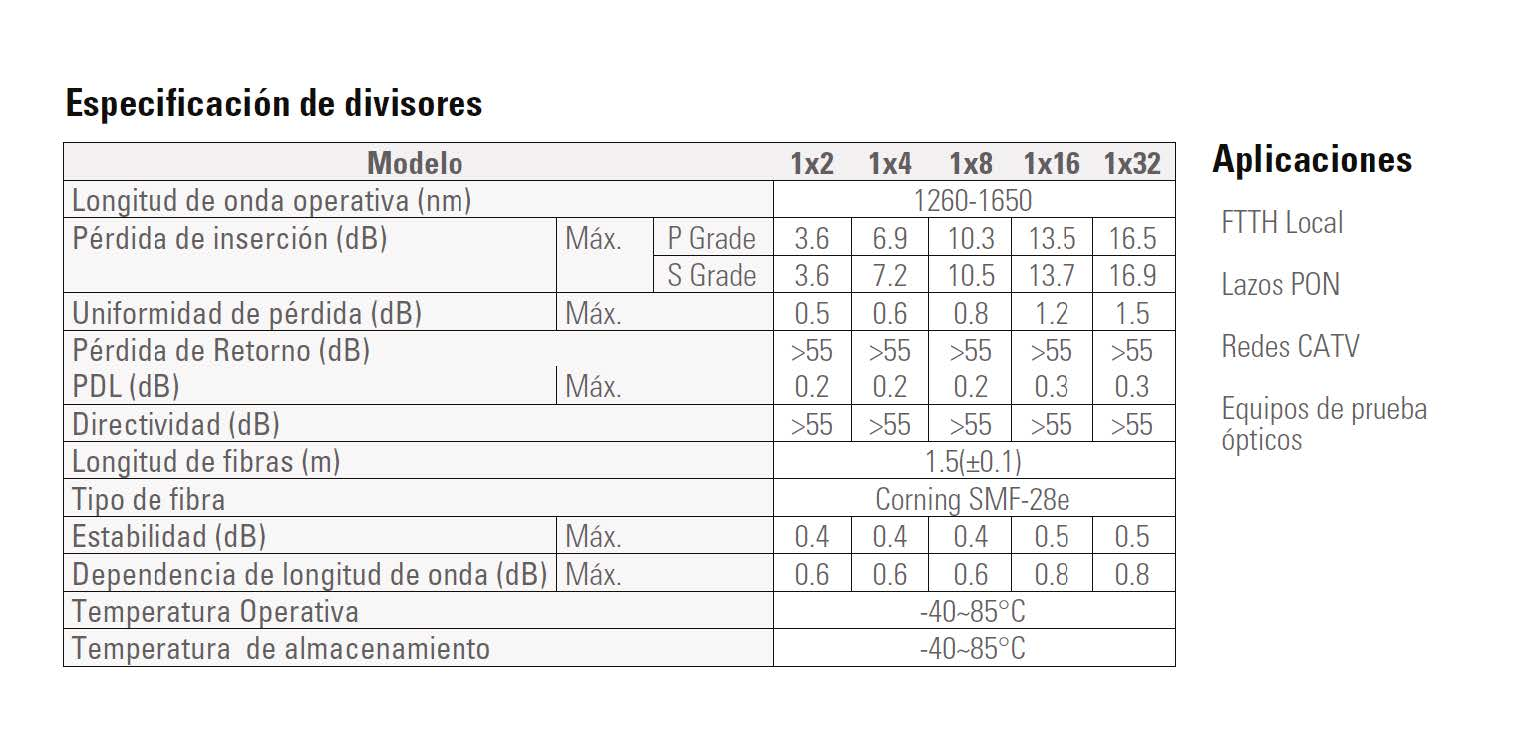
\includegraphics[width=0.8\linewidth]{fotos_ema/splitters_mach.jpg}
      \caption{Características de los splitters MACH\protect\footnote{\href{https://mach.com.ar/backend/views/images/categoria/editado658.pdf}{Catálogo MACH}}.}
      \label{fig:splitters_mach}
    \end{figure}
 
    \item  KOC, presenta las características presentadas en la Fig. \ref{fig:splitters_koc}.
    
    \begin{figure}[htbp]
      \centering
      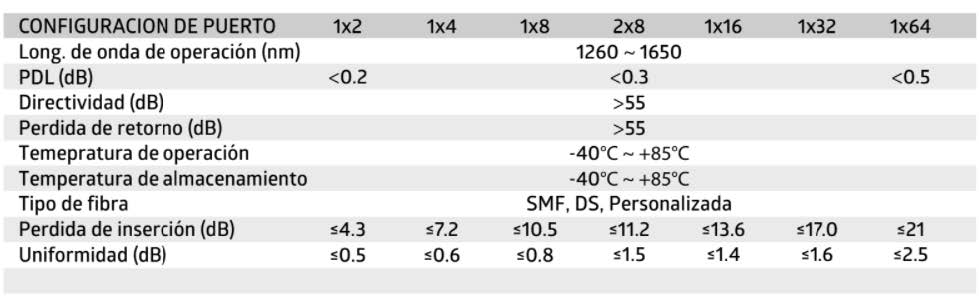
\includegraphics[width=0.8\linewidth]{fotos_ema/splitters_koc.jpg}
      \caption{Características de los splitters KOC.}
      \label{fig:splitters_koc}
    \end{figure}

    \end{itemize}

\end{document}